\documentclass[../main.tex]{subfiles}

\begin{document}

\chapter{代码主体结构}
\vspace{-2cm}

在本章节中,我们将对 BasicSR 代码框架进行一个整体介绍,主要包括以下内容:整体框架 (第\ref{code_structure:overview}小节)、注册器机制 (第\ref{code_structure:register}小节)、配置文件 (第\ref{code_structure:config}小节)、数据 (第\ref{code_structure:data}小节)、模型 (第\ref{code_structure:model}小节)、网络结构 (第\ref{code_structure:arch}小节)、损失函数 (第\ref{code_structure:loss}小节)、算子 (第\ref{code_structure:ops}小节)、日志系统  (第\ref{code_structure:logger}小节) 等。通过阅读本章,你将对 BasicSR 有进一步的认识,理解其模块之间的相互关系、以及模块内部的核心工作原理。但我们不对具体函数和代码做具体介绍。如果需要具体函数和代码的介绍,请查阅 BasicSR 的在线 API 文档 (\url{https://basicsr.readthedocs.io/en/latest/})。

% ------------------------------------------------------------------------------
\section{整体框架} \label{code_structure:overview}

对于基于深度学习的算法框架,其核心的组成部分包括:\textbf{数据、模型、损失函数、训练}。BasicSR 框架也是大致根据以上部分撰写而成的。下图概括了 BasicSR 的整体组成框架:

\begin{figure}[htbp]
    \begin{center}
        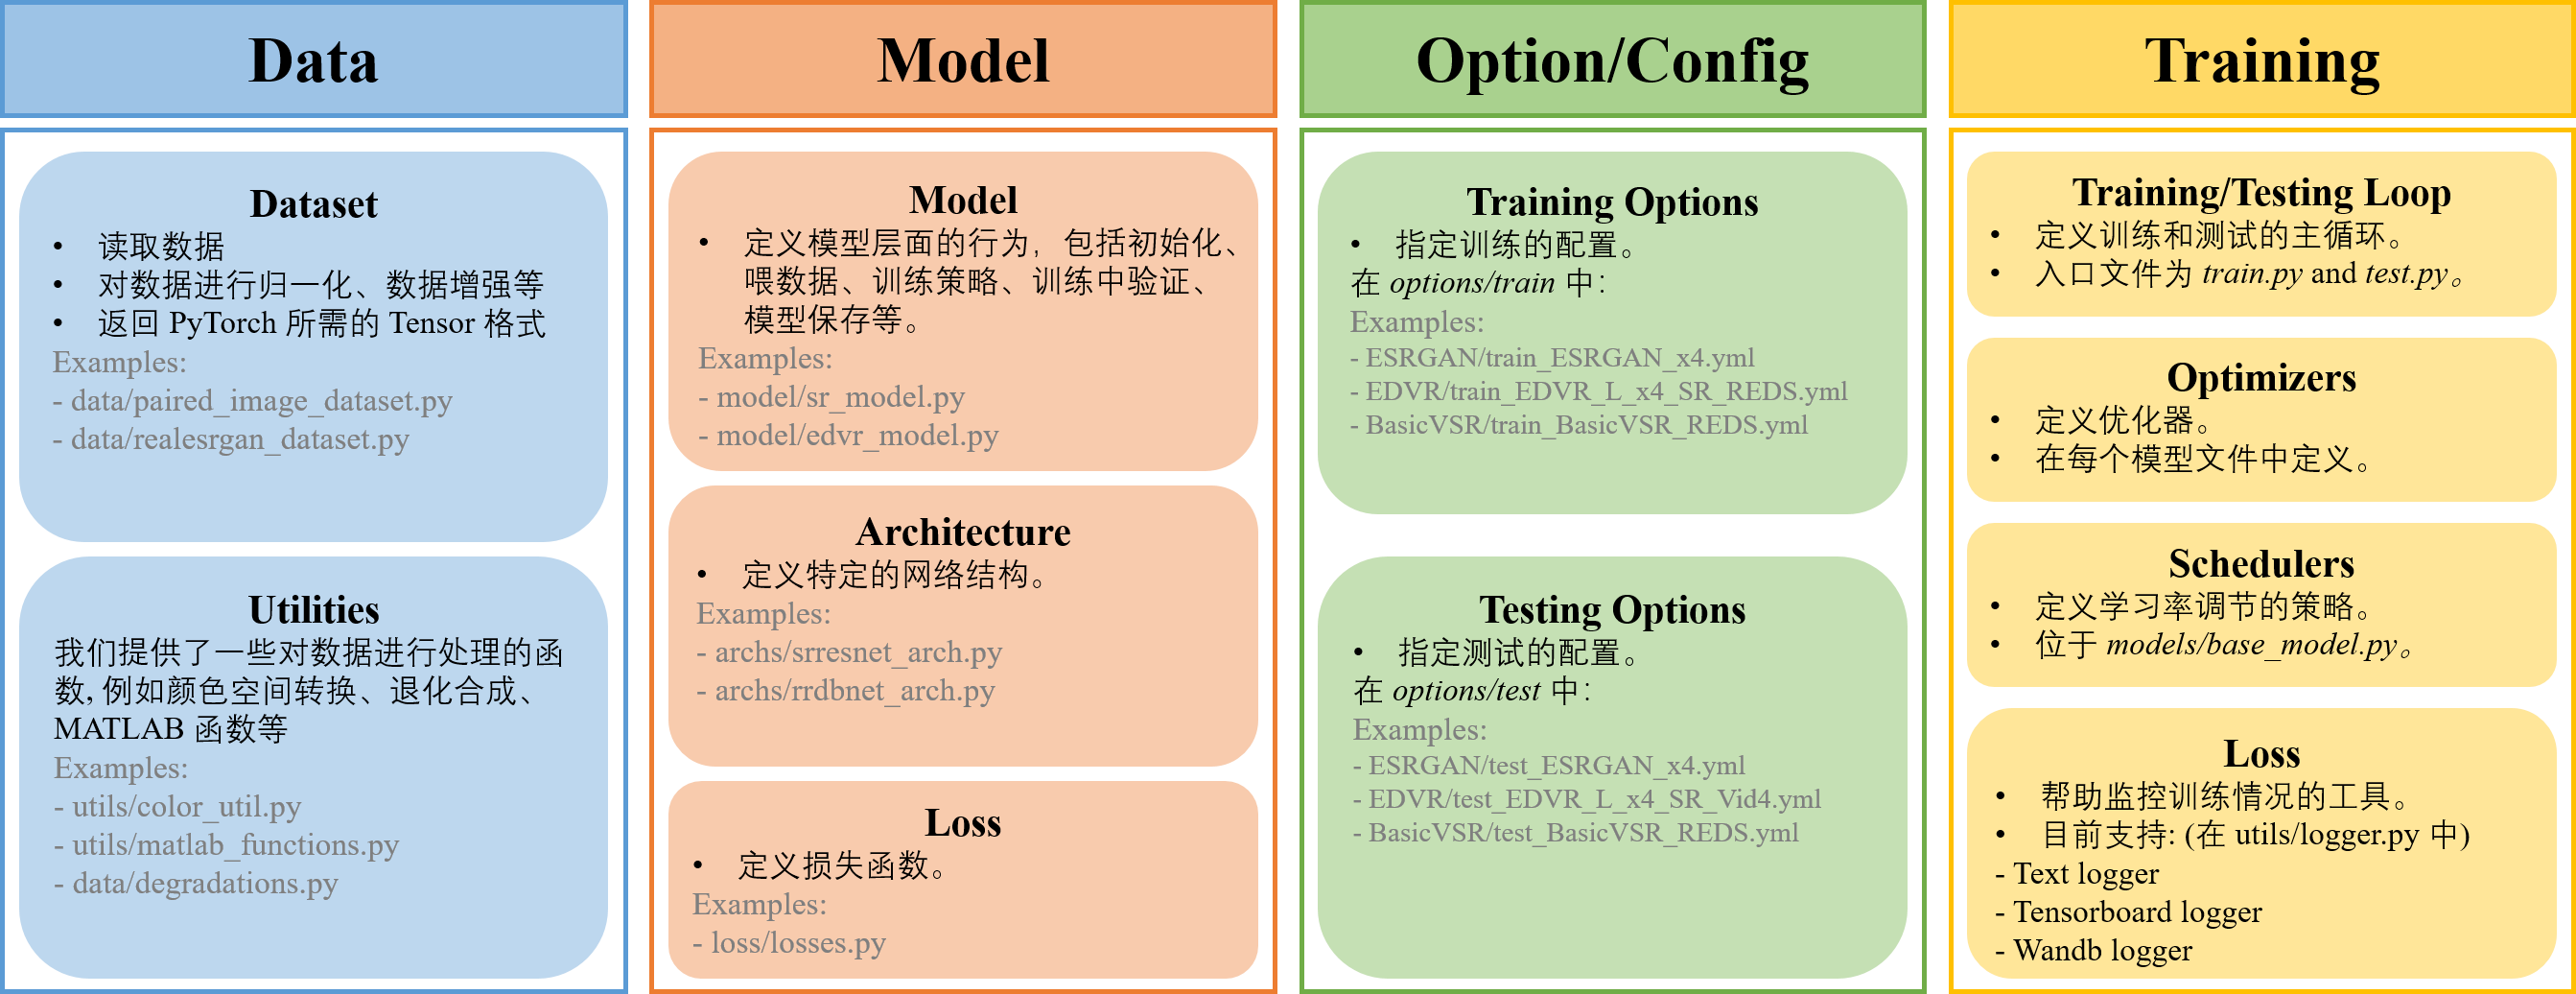
\includegraphics[width=1\linewidth]{figures/code_structure_overview.png}
    \end{center}
    \caption{BasicSR 代码整体框架}
    \label{fig:main_framework}
\end{figure}

\begin{itemize}
    \item 数据 (Data):这个部分主要定义了 Dataset 和 Data Loader 文件, 放在了 \href{https://github.com/XPixelGroup/BasicSR/tree/master/basicsr/data}{basicsr/data} 目录下。Dataset 用于读取和预处理数据,包括图像读取、归一化 (normalization)、数据增强 (augmentation) 以及封装为 PyTorch Tensor 等。同时,我们也提供了一些辅助函数,帮助使用者自定义自己的数据预处理功能,例如图像色彩空间转换、常用 MATLAB 函数的 Python 版本、常用的图像退化模型 (degradation model) 等。详细说明参见章节\ref{code_structure:data}:\nameref{code_structure:data}

    \item 模型 (Model):在 \href{https://github.com/XPixelGroup/BasicSR/tree/master/basicsr/models}{basicsr/models} 目录下,我们提供了常用的模型文件。这些模型文件主要用于定义网络结构与初始化、输入输出数据、一次 forward 的训练过程、保存加载模型等。在 \href{https://github.com/XPixelGroup/BasicSR/tree/master/basicsr/archs}{basicsr/archs} 目录下,我们提供了常用的网络结构模型文件,包括 SRResNet、ESRGAN、RCAN、SwinIR、EDVR、BasicVSR 等。在 \href{https://github.com/XPixelGroup/BasicSR/tree/master/basicsr/losses}{basicsr/losses} 文件夹中,我们提供了常用的损失函数,例如 L1/L2 loss、perceptual loss、GAN loss 等。详细说明参见章节\ref{code_structure:model}:\nameref{code_structure:model}、章节\ref{code_structure:arch}:\nameref{code_structure:arch}、章节\ref{code_structure:loss}:\nameref{code_structure:loss}

    \item 配置 (Option):配置文件放到 \href{https://github.com/XPixelGroup/BasicSR/tree/master/options}{option} 目录下。我们提供了常用模型的训练和测试配置文件。我们使用 \href{https://yaml.org/}{YAML} 来作为配置文件的语言。修改这些 yml 文件可以简易地调整训练过程中的各种超参数。详细说明参见章节\ref{code_structure:register}:\nameref{code_structure:register}和章节\ref{code_structure:config}:\nameref{code_structure:config}

    \item 训练 (Training):这一部分主要涉及训练的策略和记录训练日志。\href{https://github.com/XPixelGroup/BasicSR/blob/master/basicsr/train.py}{basicsr/train.py} 和 \href{https://github.com/XPixelGroup/BasicSR/blob/master/basicsr/test.py}{basicsr/test.py} 是启动模型训练和测试的入口文件,其中定义了训练和测试的 main loop。常见优化器 (optimizer) 的定义可以在 \href{https://github.com/XPixelGroup/BasicSR/blob/master/basicsr/models/base_model.py}{models/base\_model.py} 文件中的 \texttt{get\_optimizer} 函数中找到。学习率的调度策略在 \href{https://github.com/XPixelGroup/BasicSR/blob/master/basicsr/models/base_model.py}{models/base\_model.py}  文件中的 \texttt{setup\_schedulers} 函数中定义。为了方便追踪记录训练的过程,我们提供了相应的 logger 工具,支持直接 print 到屏幕、Tensorboard、Wandb等多种方式,具体代码可以在 \href{https://github.com/XPixelGroup/BasicSR/blob/master/basicsr/utils/logger.py}{basicsr/utils/logger.py} 中找到。详细说明参见章节\ref{code_structure:logger}:\nameref{code_structure:logger}

    \item 详细的代码接口文档可以在 \url{http://basicsr.readthedocs.io} 查询
\end{itemize}

\begin{note} % ---------------- Note block ---------------- %
    \textbf{BasicSR 目录说明}

    你可以在章节\ref{getting_start:content-overview}:\nameref{getting_start:content-overview} 查看到详细的 BasicSR 目录说明。
\end{note}
% ------------------------------------------------------------------------------
\section{动态实例化与 REGISTER 注册机制}\label{code_structure:register}

% ----------------------------------
\subsection{REGISTER 注册机制}\label{code_structure:register_intro}

首先,来看我们的目的:当我们新写了类 (Class) 或函数时,我们希望可直接在配置文件中指定,然后程序会根据配置文件的类名或函数名,自动查找并实例化。
以开发新的网络结构为例,我们会做以下几件事:
\begin{enumerate}
    \item 写具体的网络结构,它往往是一个Class,并且往往是一个单独的文件
    \item 在配置文件中会指定我们使用哪一个网络结构,往往是通过 Class name 指定
    \item 在训练过程的某一个地方,程序会根据配置文件指定的 Class name,自动实例化相关的类
\end{enumerate}

这里说的 REGISTER 注册机制就是来更简洁地实现上面的第三个步骤的。因为其能够根据配置文件动态地实例化所需要的类或函数,因此这个过程被称为动态实例化 (Dynamic Instantiation)。

BasicSR 的 Register 注册机制参考了 FacebookResearch 的 \href{https://github.com/facebookresearch/fvcore}{fvcore} 仓库的函数,定义了 Registry 类。详细代码可查看 \href{https://github.com/XPixelGroup/BasicSR/blob/master/basicsr/utils/registry.py}{basicsr/utils/registry.py}。它主要有两个函数:register() 和 get()。

\begin{minted}[xleftmargin=20pt,linenos,bgcolor=bg,breaklines]{python}
class Registry():
    """
    The registry that provides name -> object mapping, to support third-party users' custom modules.
    """
    def __init__(self, name):
        self._name = name
        self._obj_map = {}

    def _do_register(self, name, obj, suffix=None):
        ...
        self._obj_map[name] = obj

    def register(self, obj=None, suffix=None):
        # register() 函数主要用来注册一个实现的类或函数
        if obj is None:
            # used as a decorator
            def deco(func_or_class):
                name = func_or_class.__name__
                self._do_register(name, func_or_class, suffix)
                return func_or_class

            return deco

        # used as a function call
        name = obj.__name__
        self._do_register(name, obj, suffix)

    def get(self, name, suffix='basicsr'):
        # get() 函数主要用来根据配置文件中的类名或函数名来查找对应的实例
        ret = self._obj_map.get(name)
        if ret is None:
            ret = self._obj_map.get(name + '_' + suffix)
        ...
        return ret
\end{minted}

\subsubsection{如何注册新的类?}\label{code_structure:how_to_register}

在 BasicSR 中,我们定义了五个 REGISTER ,相关定义在 \href{https://github.com/XPixelGroup/BasicSR/blob/master/basicsr/utils/registry.py}{basicsr/utils/registry.py} 中:
\begin{minted}[xleftmargin=20pt,linenos,bgcolor=bg,breaklines]{python}
DATASET_REGISTRY = Registry('dataset')
ARCH_REGISTRY = Registry('arch')
MODEL_REGISTRY = Registry('model')
LOSS_REGISTRY = Registry('loss')
METRIC_REGISTRY = Registry('metric')
\end{minted}

需要注册的时候,我们
\begin{enumerate}
    \item import 相关的注册器,比如 ARCH\_REGISTRY
    \item 使用 Python 装饰器,即在类/函数前面加上 \texttt{@ARCH\_REGISTRY.register()}
\end{enumerate}
以网络结构 RRDBNet 为例:

\begin{minted}[xleftmargin=20pt,linenos,bgcolor=bg,breaklines]{python}
from basicsr.utils.registry import ARCH_REGISTRY  # import 相关的注册器
from .arch_util import default_init_weights, make_layer, pixel_unshuffle

@ARCH_REGISTRY.register()  # 使用 Python 装饰器
class RRDBNet(nn.Module):
    def __init__(self):
        super(RRDBNet, self).__init__()
        ...
\end{minted}

这样 RRDBNet 这个类就被注册上了。

\subsubsection{如何使用已注册的类?}\label{code_structure:how_to_use_registerd}

当我们需要使用的时候,只需要在配置文件中配置,相关代码会自动实例化所需的类。

还是以使用 RRDBNet 网络结构为例。我们在配置文件中指定了网络结构的类型为 RRDBNet。
\begin{minted}[xleftmargin=20pt,linenos,bgcolor=bg,breaklines]{yaml}
# network structures
network_g:
  type: RRDBNet
  num_in_ch: 3
  num_out_ch: 3
  num_feat: 64
  num_block: 23
\end{minted}

模型文件 \href{https://github.com/XPixelGroup/BasicSR/blob/master/basicsr/models/sr_model.py}{basicr/models/sr\_models.py} 中的函数 \texttt{build\_network(opt['network\_g'])} 便会根据配置文件 build 网络结构。
\begin{minted}[xleftmargin=20pt,linenos,bgcolor=bg,breaklines]{python}
class SRModel(BaseModel):
    """Base SR model for single image super-resolution."""

    def __init__(self, opt):
        super(SRModel, self).__init__(opt)

        # define network
        self.net_g = build_network(opt['network_g'])  # 调用建构网络结构的函数
        self.net_g = self.model_to_device(self.net_g)
        self.print_network(self.net_g)
\end{minted}

而 \texttt{build\_network} 函数就会从 ARCH\_REGISTRY 中找到已经被注册的 RRDBNet 进行实例化。 \texttt{build\_network} 函数所在位置 \href{https://github.com/XPixelGroup/BasicSR/blob/master/basicsr/archs/\_\_init\_\_.py}{basicsr/archs/\_\_init\_\_.py}

\begin{minted}[xleftmargin=20pt,linenos,bgcolor=bg,breaklines]{python}
def build_network(opt):
    opt = deepcopy(opt)
    network_type = opt.pop('type')
    net = ARCH_REGISTRY.get(network_type)(**opt)  # 实例化的核心函数。从 ARCH_REGISTRY 找到已被注册的类进行实例化
    logger = get_root_logger()
    logger.info(f'Network [{net.__class__.__name__}] is created.')
    return net
\end{minted}

% ----------------------------------
\subsection{自动扫描并 import 注册的类/函数}\label{code_structure:auto_import}

上面讲了 REGISTER 注册机制,但还有一个问题:这个类/函数还需要被 Python 程序感知到。目前的类/函数只是在一个文件中写了,但是 Python 程序并没有 import 进来。

这个问题的解决方法:一般是在 \_\_init\_\_.py 文件中写 import 语句,比如在 mmediting 中定义了网络结构后,还需要在 sr\_backbones/\_\_init\_\_.py 中添加这样的语句:
\begin{minted}[xleftmargin=20pt,linenos,bgcolor=bg,breaklines]{python}
from .basicvsr_net import BasicVSRNet
from .edsr import EDSR
from .edvr_net import EDVRNet
from .rrdb_net import RRDBNet
from .sr_resnet import MSRResNet
\end{minted}

它需要在 \_\_init\_\_.py 中把写好的网络结构显示地 import 进来。
但这样很麻烦:每写一个新的网络结构,我们就要去修改 \_\_init\_\_.py,很多时候容易忘记。
最早开发 mmediting 的时候就感觉这个很繁琐。
本着偷懒的原则,在 BasicSR 中就找了一个省事的办法。

但我们新建一个文件,就以 \texttt{\_arch.py} 结尾。通过扫描特定文件的方式来进行自动 import。
比如,对于网络结构,我们在 \href{https://github.com/XPixelGroup/BasicSR/blob/master/basicsr/archs/\_\_init\_\_.py}{basicsr/archs/\_\_init\_\_.py} 中定义了:

\begin{minted}[xleftmargin=20pt,linenos,bgcolor=bg,breaklines]{python}
# automatically scan and import arch modules for registry
# scan all the files under the 'archs' folder and collect files ending with '_arch.py'
arch_folder = osp.dirname(osp.abspath(__file__))
arch_filenames = [osp.splitext(osp.basename(v))[0] for v in scandir(arch_folder) if v.endswith('_arch.py')]
# import all the arch modules
_arch_modules = [importlib.import_module(f'basicsr.archs.{file_name}') for file_name in arch_filenames]
\end{minted}

我们可以看到,程序会自动扫描以 \texttt{\_arch.py} 的文件,然后 import 相关文件。这样就把所有注册的网络结构类都 import 进去啦。

类似的,DATASET,ARCH,MODEL,LOSS 都在相关的 \_\_init\_\_.py 文件中定义了扫描并自动 import 的操作。

总结一下,当我们在新开发网络结构时 (其他模块也类似),只要做两件事,修改两个文件就好了。BasicSR 背后的动态实例化和 REGISTRY 机制会帮你完成剩下的事。
 \begin{enumerate}
    \item 写一个单独的网络结构文件 (以 \_arch.py 结尾)。在写好的 Class 前加上 @ARCH\_REGISTRY.register() 装饰器
    \item 在配置文件中指定使用哪一个网络结构,即上面的 Class name
\end{enumerate}

\subsubsection{文件后缀名的约定}\label{code_structure:file_suffix_convention}

\begin{table}[h]
    \centering
    \begin{tabular}{|c|c|c|c|}
        \hline
        \textbf{Model} & \textbf{Register} & \textbf{File Suffix} & \textbf{Example}                       \\ \hline
        data           & DATASET\_REGISTRY & \_dataset.py         & basicsr/data/paired\_image\_dataset.py \\ \hline
        arch           & ARCH\_REGISTRY    & \_arch.py            & basicsr/archs/srresnet\_arch.py        \\ \hline
        model          & MODEL\_REGISTRY   & \_arch.py            & basicsr/models/sr\_model.py            \\ \hline
        loss           & LOSS\_REGISTRY    & \_loss.py            & basicsr/losses/gan\_loss.py            \\ \hline
    \end{tabular}
    \caption{文件后缀名的约定}
\end{table}

\begin{hl} % ---------------- Highlight block ---------------- %
    \textbf{注意}

    \begin{enumerate}
        \item 上面的文件后缀只用在需要的文件中,其他文件命名尽量避免使用以上的后缀
        \item 注册的类名或函数名不能重复,否则会报错
    \end{enumerate}
\end{hl}

\begin{hl} % ---------------- Highlight block ---------------- %
    \textbf{METRIC 稍有特殊}

    我们定义了 METRIC\_REGISTRY,它在用法上和其他类一样,但是它是根据\textbf{函数名}来调用相对应的函数。

    因为 metric 我们相对改动少,所以我们没有采用自动扫描文件再 import 的方式,而是保留了在\href{https://github.com/XPixelGroup/BasicSR/blob/master/basicsr/metrics/\_\_init\_\_.py}{basicsr/metrics/\_\_init\_\_.py} 中 import 的方式
\end{hl}

\subsubsection{避免类名/函数名出现重名问题}\label{code_structure:avoid_repeated_name}

Register 机制会自动检测出重名的类/函数,然后抛出错误:\texttt{An object named xxx was already registered in yyy registry!}。
这是特意设计的,以减少 bug 。因为如果重名的类,在实例化的时候,就不能确定程序到底实例化的是哪一个类。

但是有有一种情况下,Register 的重名检查机制反而会掣肘开发。

当我们在 BasicSR 里面定义了一个类,比如 \href{https://github.com/XPixelGroup/BasicSR/blob/master/basicsr/data/realesrgan\_dataset.py}{basicsr/data/realesrgan\_dataset.py} 中的 \texttt{RealESRGANDataset} 类。
而在 \href{https://github.com/xinntao/Real-ESRGAN}{Real-ESRGAN GitHub repo} 中,我们是把 basicsr 当作一个 package 来使用,然后又定义了一遍 \texttt{RealESRGANDataset} 类。这个时候,原来 BasicSR 代码中的类和后面开发的 Real-ESRGAN 代码中的类就有重名了。

这个情况下,我们约定在 BasicSR 对应的类中的注册器中,传入 \texttt{basicsr} 的参数,以指示这个类是 BasicSR 中定义的,以示区分。
其中这里的 \texttt{basicsr} 是关键词,注意使用其他词是不会被识别的。
\begin{minted}[xleftmargin=20pt,linenos,bgcolor=bg,breaklines]{python}
@DATASET_REGISTRY.register(suffix='basicsr')  # 我们在类名中传入后缀 suffix,以指示这是在 BasicSR repo 中定义的
class RealESRGANDataset(data.Dataset):
    """Dataset used for Real-ESRGAN model:
    """
    ...
\end{minted}

这个具体在 \href{https://github.com/XPixelGroup/BasicSR/blob/master/basicsr/utils/registry.py}{basicsr/utils/registry.py} 的代码如下:
\begin{minted}[xleftmargin=20pt,linenos,bgcolor=bg,breaklines]{python}
def get(self, name, suffix='basicsr'):
    ret = self._obj_map.get(name)
    if ret is None:
        ret = self._obj_map.get(name + '_' + suffix)
        print(f'Name {name} is not found, use name: {name}_{suffix}!')
    if ret is None:
        raise KeyError(f"No object named '{name}' found in '{self._name}' registry!")
    return ret
\end{minted}
它实现的逻辑如下:
 \begin{enumerate}
    \item 如果 get 函数指定了 suffix,则会优先找带有 suffix 的类/函数
    \item 一般我们的 get 函数都不会指定 suffix。这样的情况,程序优先找自己实现的 (比如 Real-ESRGAN 代码库中的) 类/函数
    \item 如果在自己实现的类/函数中没有找到,则会找 BasicSR 官方库中的实现的相同名字的类
\end{enumerate}

% ------------------------------------------------------------------------------
\section{配置(Options)}\label{code_structure:config}

在这个章节,我们先简单介绍一下实验命名的约定 (第\ref{code_structure:name_convention}小节);然后通过例子介绍训练和测试的配置文件 (第\ref{code_structure:config_example}小节)。

% ----------------------------------
\subsection{实验命名与 debug 模式}\label{code_structure:name_convention_debug}

\subsubsection{实验命名}\label{code_structure:name_convention}

我们推荐对实验名字进行有意义的命名,方便后续的实验以及进行多组实验对比。

我们以 \texttt{001\_MSRResNet\_x4\_f64b16\_DIV2K\_1000k\_B16G1\_wandb} 为例:

\begin{itemize}
    \item \texttt{001}: 我们一般给实验进行数字打头的标号, 方便进行实验管理
    \item \texttt{MSRResNet}: 模型名称, 这里指代 Modified SRResNet
    \item \texttt{x4\_f64b16}: 重要配置参数, 这里表示放大4倍; 中间feature通道数是64, 使用了16个Residual Block
    \item \texttt{DIV2K}: 训练数据集是 DIV2K
    \item \texttt{1000k}: 训练了1000K iterations
    \item \texttt{B16G1}: Batch size 为16, 使用一卡 GPU 训练
    \item \texttt{wandb}: 使用了 wandb, 训练过程上传到了 wandb 云服务器
\end{itemize}

\subsubsection{Debug 模式}\label{code_structure:debug_mode}

正式训练之前,你可以用 debug 模式检查是否正常运行。在 debug 模式下:
\begin{itemize}
    \item 程序会在每次 iteration 下都打印日志,并且经过8次 iterations 后,便会进入 validation 阶段。这样可以快速方便地查看代码是否可以正常运行,而不用实际训练。毕竟实际训练可能很慢,等半天后,发现程序崩溃了,而原因是 validation 中有 bug
    \item 在 debug 模式中,并不会使用 tensorboard logger 和 wandb logger,以保证日志文件的简洁性
\end{itemize}

\textbf{如何进入 debug 模式?}

\begin{enumerate}[方式 1.]
    \item 在命令行最后加入 ‘\textbf{-{}-debug}’。比如:
          \begin{minted}[xleftmargin=20pt,linenos,breaklines,bgcolor=bg]{python}
 python basicsr/train.py -opt options/train/SRResNet_SRGAN/train_MSRResNet_x4.yml --debug
    \end{minted}
    \item 在配置文件 yml 文件的 name 中添加 ‘debug’ 字符。只要在实验名字中有 ‘\uline{debug}’ 字样, 则会进入 debug 模式。
\end{enumerate}

% ----------------------------------
\subsection{配置文件简要说明}\label{code_structure:config_example}

在 BasicSR 中我们使用 \href{https://yaml.org/}{YAML} 来作为配置文件的语言。

训练的配置文件在 \href{https://github.com/XPixelGroup/BasicSR/tree/master/options/train}{options/train} 中,测试的配置文件在 \href{https://github.com/XPixelGroup/BasicSR/tree/master/options/test}{options/test} 中。
通过 option 配置文件,我们可以设置实验名、选择模型、指定 GPU、指定数据路径、选择网络结构、配置训练策略等。我们在第\ref{code_structure:train_config}小节介绍训练配置文件例子,在第\ref{code_structure:test_config}小节介绍测试配置文件例子。

\textbf{配置文件的解析}在 \href{https://github.com/XPixelGroup/BasicSR/blob/master/basicsr/utils/options.py}{basicsr/utils/options.py} 的 \texttt{parse\_options} 中实现。这个过程将 YAML 文件解析成 Python 的 dict 类型,并根据需要做出调整 (比如 debug 模式下的特殊配置等)。读者可以在章节\ref{getting_start:entrance}:\nameref{getting_start:entrance} 和对应代码中找到解释和具体实现。

\subsubsection{训练配置文件例子}\label{code_structure:train_config}

下面,我们以 \href{https://github.com/XPixelGroup/BasicSR/blob/master/options/train/SRResNet_SRGAN/train_MSRResNet_x4.yml}{train\_MSRResNet\_x4.yml} 为例,简单说明训练配置文件的每个部分。我们先把配置文件贴出来,在后面附上解释。然后在说明框内会列举相关的要点。为方便说明,整个配置文件会被分散成不同的板块来讲解。

\begin{minted}[xleftmargin=20pt,breaklines,bgcolor=bg]{python}
# Modified SRResNet w/o BN from:
# Photo-Realistic Single Image Super-Resolution Using a Generative Adversarial Network

# ----------- Commands for running
# ----------- Single GPU with auto_resume
# PYTHONPATH="./:${PYTHONPATH}"  CUDA_VISIBLE_DEVICES=0 python basicsr/train.py -opt options/train/SRResNet_SRGAN/train_MSRResNet_x4.yml --auto_resume

# general settings - 这块为通用设置
name: 001_MSRResNet_x4_f64b16_DIV2K_1000k_B16G1_wandb  # 实验名称, 若实验名字中有debug字样, 则会进入debug模式
model_type: SRModel  # 使用的 model 类型
scale: 4  # 输出比输入的倍数, 在SR中是放大倍数; 若有些任务没有这个配置, 则写1
num_gpu: 1  # 指定使用的 GPU 卡数
manual_seed: 0  # 指定随机种子
\end{minted}

\begin{exampleBox}[righthand ratio=0.00, sidebyside, sidebyside align=center, lower separated=false]{通用配置}
    \begin{itemize}
        \item 在配置文件的最开始,会有简单的说明,以及默认的运行命令。运行命令的 \texttt{auso\_resume} 表示自动从断点接着训练 (详见章节\ref{code_structure:howto_resume}:\nameref{code_structure:howto_resume})
        \item 常见模型 (Model) 的定义在 \href{https://github.com/XPixelGroup/BasicSR/tree/master/basicsr/models}{models} 目录中。详细说明参见章节\ref{code_structure:model}:\nameref{code_structure:model}
        \item \texttt{num\_gpu}:\textbf{0 表示 使用CPU,\texttt{auto} 表示自动从可用 GPU 块数推断}
    \end{itemize}
\end{exampleBox}

\begin{minted}[xleftmargin=20pt,bgcolor=bg,breaklines]{python}
# dataset and data loader settings
datasets:  # 这块是 dataset 的配置
  train:  # 训练 dataset 的配置
    name: DIV2K  # 自定义的数据集名称
    type: PairedImageDataset  # 读取数据的 Dataset 类
    # 以下属性是灵活的, 可在相应类的说明文档中获得。新加的数据集可根据需要添加
    dataroot_gt: datasets/DF2K/DIV2K_train_HR_sub  #  GT (Ground-Truth) 图像的文件夹路径
    dataroot_lq: datasets/DF2K/DIV2K_train_LR_bicubic_X4_sub  # LQ (Low-Quality) 输入图像的文件夹路径
    meta_info_file: basicsr/data/meta_info/meta_info_DIV2K800sub_GT.txt  # 预先生成的 meta_info 文件
    # (for lmdb)
    # dataroot_gt: datasets/DIV2K/DIV2K_train_HR_sub.lmdb
    # dataroot_lq: datasets/DIV2K/DIV2K_train_LR_bicubic_X4_sub.lmdb
    filename_tmpl: '{}'  # 文件名字模板, 一般LQ文件会有类似 '_x4' 这样的文件后缀, 这个就是来处理GT和LQ文件后缀不匹配的问题的
    io_backend:  # IO 读取的 backend
      type: disk  # disk 表示直接从硬盘读取
      # (for lmdb)
      # type: lmdb

    gt_size: 128  # 训练阶段裁剪 (crop) 的GT图像的尺寸大小,即训练的 label 大小
    use_hflip: true  # 是否开启水平方向图像增强 (随机水平翻转图像)
    use_rot: true  # 是否开启旋转图像增强 (随机旋转图像)

    # data loader - 下面这块是 data loader 的设置
    num_worker_per_gpu: 6  # 每一个 GPU 的 data loader 读取进程数目
    batch_size_per_gpu: 16  # 每块 GPU 上的 batch size
    dataset_enlarge_ratio: 100  # 放大 dataset 的长度倍数 (默认为1)。可以扩大一个 epoch 所需 iterations
    prefetch_mode: ~  # 预先读取数据的方式
\end{minted}
\begin{exampleBox}[righthand ratio=0.00, sidebyside, sidebyside align=center, lower separated=false]{数据读取相关配置}
    \begin{itemize}
        \item 常见数据 (dataset) 的定义在 \href{https://github.com/XPixelGroup/BasicSR/blob/master/basicsr/data}{basicsr/data} 目录中。详细说明参见章节\ref{code_structure:data}:\nameref{code_structure:data}
        \item data loader 定义在 \href{https://github.com/XPixelGroup/BasicSR/blob/master/basicsr/data/__init__.py}{basicsr/data/\_\_init\_\_.py} 文件中
        \item meta\_info\_file:细节请参看章节\ref{data_preparation:meta_info}:\nameref{data_preparation:meta_info} \todo{更新链接}
        \item io\_backend:细节请参看章节\ref{data_preparation:meta_info}:\nameref{data_preparation:meta_info} \todo{更新链接}
        \item dataset\_enlarge\_ratio:它代表了手工扩大 dataset 的倍率。例如,如果训练数据集有15张图,设置 dataset\_enlarge\_ratio 为100,那么程序会重复读取这些图片100次,这样一个 epoch 下来,便会读取1500张图 (事实上是重复读的)。这个方法经常用来加速 data loader, 因为在有的机器上,一个 epoch 结束,会重启进程,导致拖慢训练
        \item prefetch\_mode:,\textbf{默认为 None,即 $\sim$。\texttt{cpu} 表示使用 CPU prefetcher。\texttt{cuda} 表示使用 CUDA prefetcher。它会多占用一些GPU显存. 注意: 这个模式下, 一定要设置 \texttt{pin\_memory=True}}。详情参见章节\ref{code_structure:dataset_prefecth}:\nameref{code_structure:dataset_prefecth}
    \end{itemize}
\end{exampleBox}

\begin{minted}[xleftmargin=20pt,bgcolor=bg,breaklines]{python}
  val:  # validation 数据集的设置
    name: Set5  # 数据集名称
    type: PairedImageDataset  # 数据集的类型
    # 以下属性是灵活的, 类似训练数据集
    dataroot_gt: datasets/Set5/GTmod12
    dataroot_lq: datasets/Set5/LRbicx4
    io_backend:
      type: disk

  val_2:  # 另外一个 validation 数据集
    name: Set14
    type: PairedImageDataset
    dataroot_gt: datasets/Set14/GTmod12
    dataroot_lq: datasets/Set14/LRbicx4
    io_backend:
      type: disk
\end{minted}

\begin{exampleBox}[righthand ratio=0.00, sidebyside, sidebyside align=center, lower separated=false]{validation 配置}
    \begin{itemize}
        \item 这里使用了两个 validation sets,它们通过关键字 \texttt{val},\texttt{val\_2} 来区分。如果有更多的 validation sets,可以通过 \texttt{val\_3}, \texttt{val\_4} ... 来区分
    \end{itemize}
\end{exampleBox}

\begin{minted}[xleftmargin=20pt,bgcolor=bg,breaklines]{python}
# network structures - 网络结构的设置
network_g:  # 网络 g 的设置
  type: MSRResNet  # 网络结构 (Architecture) 的类型
  # 以下属性是灵活且特定的, 可在相应类的说明文档中获得
  num_in_ch: 3  # 模型输入的图像通道数
  num_out_ch: 3  # 模型输出的图像通道数
  num_feat: 64  # 模型内部的 feature map 通道数
  num_block: 16  # 模型内部基础模块的堆叠数
  upscale: 4  # 上采样倍数
\end{minted}

\begin{exampleBox}[righthand ratio=0.00, sidebyside, sidebyside align=center, lower separated=false]{网络结构相关配置}
    \begin{itemize}
        \item 常见网络结构 (arch) 的定义在 \href{https://github.com/XPixelGroup/BasicSR/tree/master/basicsr/archs}{archs} 目录下。详细说明参见章节\ref{code_structure:arch}:\nameref{code_structure:arch}
        \item 如果模型需要使用多个网络,我们一般以 \texttt{network\_} 打头来命名。比如 我们需要一个 discriminator,命名为  \texttt{network\_d}
    \end{itemize}
\end{exampleBox}

\begin{minted}[xleftmargin=20pt,bgcolor=bg,breaklines]{python}
# path
path:  # 以下为路径和与训练模型、重启训练的设置
  pretrain_network_g: ~  # 预训练模型的路径, 需要以 pth 结尾的模型
  param_key_g: params  # 读取的预训练的参数 key。若需要使用 EMA 模型,需要改成 params_ema
  strict_load_g: true  # 是否严格地根据参数名称一一对应 load 模型参数。如果选择 false,那么模型对于找不到的参数,会随机初始化;如果选择 true,假如存在不对应的参数,会报错提示
  resume_state: ~  # 重启训练的 state 路径, 在 experiments/exp_name/training_states 目录下
\end{minted}

\begin{exampleBox}[righthand ratio=0.00, sidebyside, sidebyside align=center, lower separated=false]{模型路径相关配置}
    \begin{itemize}
        \item resume\_state设置后, 会覆盖 pretrain\_network\_g 的设定
        \item 对于 resume,更多信息可以参考章节\ref{code_structure:howto_resume}:\nameref{code_structure:howto_resume}
    \end{itemize}
\end{exampleBox}

\begin{minted}[xleftmargin=20pt,bgcolor=bg,breaklines]{python}
# training settings
train:  # 这块是训练策略相关的配置
  ema_decay: 0.999  # EMA 更新权重
  optim_g:  # 这块是优化器的配置
    type: Adam  # 选择优化器类型,例如 Adam
    # 以下属性是灵活的, 根据不同优化器有不同的设置
    lr: !!float 2e-4  # 初始学习率
    weight_decay: 0  # 权重衰退参数
    betas: [0.9, 0.99]  # Adam 优化器的 beta1 和 beta2

  scheduler:  # 这块是学习率调度器的配置
    type: CosineAnnealingRestartLR   # 选择学习率更新策略
    # 以下属性是灵活的, 根据学习率 Scheduler 的不同有不同的设置
    periods: [250000, 250000, 250000, 250000]  # Cosine Annealing 的更新周期
    restart_weights: [1, 1, 1, 1]  # Cosine Annealing 每次 Restart 的权重
    eta_min: !!float 1e-7  # 学习率衰退到的最小值

  total_iter: 1000000  # 总共进行的训练迭代次数
  warmup_iter: -1  #  warm up 的迭代次数, 如是-1, 表示没有 warm up

  # losses - 这块是损失函数的设置
  pixel_opt:  # loss 名字,这里表示 pixel-wise loss 的 options
    type: L1Loss  # 选择 loss 函数,例如 L1Loss
    # 以下属性是灵活的, 根据不同损失函数有不同的设置
    loss_weight: 1.0  # 指定 loss 的权重
    reduction: mean  # loss reduction 方式
\end{minted}

\begin{exampleBox}[righthand ratio=0.00, sidebyside, sidebyside align=center, lower separated=false]{训练策略相关配置}

    训练策略相关的配置主要分为优化器,学习率调度器,总共训练 iterations,损失函数等。
    \begin{itemize}
        \item 关于 EMA,请参考章节\ref{code_structure:ema}:\nameref{code_structure:ema}
        \item optim\_g,后缀 \texttt{\_g} 表示和 \texttt{network\_g} 中的 \texttt{\_g} 一一对应起来
        \item \texttt{lr: !!float 2e-4} 中的 \texttt{!!float} 是 YAML 语言语法,表示以 float 解释后面的数字,不然就会以文字来进行解释
        \item 常见优化器 (optimizer) 的定义可以在 \href{https://github.com/XPixelGroup/BasicSR/blob/master/basicsr/models/base_model.py}{models/base\_model.py} 文件中的 \texttt{get\_optimizer} 函数中找到
        \item 学习率的调度策略在 \href{https://github.com/XPixelGroup/BasicSR/blob/master/basicsr/models/base_model.py}{models/base\_model.py}  文件中的 \texttt{setup\_schedulers} 函数中定义
        \item 常用的损失函数可以在 \href{https://github.com/XPixelGroup/BasicSR/tree/master/basicsr/losses}{losses} 目录中定义
    \end{itemize}
\end{exampleBox}

\begin{minted}[xleftmargin=20pt,bgcolor=bg,breaklines]{python}
# validation settings
val:  # 这块是 validation 的配置
  val_freq: !!float 5e3  # validation 频率, 每隔 5000 iterations 做一次 validation
  save_img: false  # 否需要在 validation 的时候保存图片

  metrics:  # 这块是 validation 中使用的指标的配置
    psnr:  # metric 名字, 这个名字可以是任意的
      type: calculate_psnr  # 选择指标类型
      # 以下属性是灵活的, 根据不同 metric 有不同的设置
      crop_border: 4  # 计算指标时 crop 图像边界像素范围 (不纳入计算范围)
      test_y_channel: false  # 是否转成在 Y(CbCr) 空间上计算
      better: higher  # 该指标是越高越好,还是越低越好。选择 higher 或者 lower,默认为 higher
    niqe:  # 这是在 validation 中使用的另外一个指标
      type: calculate_niqe
      crop_border: 4
      better: lower  # the lower, the better
\end{minted}

\begin{exampleBox}[righthand ratio=0.00, sidebyside, sidebyside align=center, lower separated=false]{validation 相关配置}
    \begin{itemize}
        \item 关于 metrics,请参考章节\ref{metrics:}:\nameref{metrics:} \todo{更新}
        \item 指标在 \href{https://github.com/XPixelGroup/BasicSR/tree/master/basicsr/metrics}{basicsr/metrics} 目录中定义
        \item BasicSR 支持在 validation 时使用多个指标,只需要在配置文件中添加配置,比如上面的 \texttt{psnr} 和 \texttt{niqe}
    \end{itemize}
\end{exampleBox}

\begin{minted}[xleftmargin=20pt,bgcolor=bg,breaklines]{python}
# logging settings
logger:  # 这块是 logging 的配置
  print_freq: 100  # 多少次迭代打印一次训练信息
  save_checkpoint_freq: !!float 5e3  # 多少次迭代保存一次模型权重和训练状态
  use_tb_logger: true  # 是否使用 tensorboard logger
  wandb:  # 是否使用 wandb logger
    project: ~  #  wandb 的 project名字。 默认是 None, 即不使用 wandb
    resume_id: ~  # 如果是 resume, 可以输入上次的 wandb id, 则 log 可以接起来
\end{minted}

\begin{exampleBox}[righthand ratio=0.00, sidebyside, sidebyside align=center, lower separated=false]{训练日志相关配置}
    \begin{itemize}
        \item 关于 wandb,目前 wandb 只是同步 tensorboard 的内容, 因此要使用 wandb, 必须也同时使用 tensorboard。更多关于 wandb,参见章节\ref{metrics:}:\nameref{metrics:} \todo{更新}
    \end{itemize}
\end{exampleBox}

\begin{minted}[xleftmargin=20pt,bgcolor=bg,breaklines]{python}
# dist training settings
dist_params:  # distributed training 的设置, 目前只在 Slurm 训练下才需要
  backend: nccl
  port: 29500
\end{minted}

至此,我们对于训练的配置文件有了一个初步的理解了。

\subsubsection{测试配置文件例子}\label{code_structure:test_config}

我们以 \href{https://github.com/XPixelGroup/BasicSR/blob/master/options/test/SRResNet_SRGAN/test_MSRResNet_x4.yml}{test\_MSRResNet\_x4.yml} 为例,简单说明测试配置文件的每个部分。我们先把配置文件贴出来,在后面附上解释。然后在说明框内会列举相关的要点。为方便说明,整个配置文件会被分散成不同的板块来讲解。
由于测试配置文件和训练配置文件很类似,我们将简略地进行讲解。

\begin{minted}[xleftmargin=20pt,breaklines,bgcolor=bg]{python}
# ----------- Commands for running
# ----------- Single GPU
# PYTHONPATH="./:${PYTHONPATH}"  CUDA_VISIBLE_DEVICES=0 python basicsr/test.py -opt options/test/SRResNet_SRGAN/test_MSRResNet_x4.yml

# general settings
name: 001_MSRResNet_x4_f64b16_DIV2K_1000k_B16G1_wandb  # 实验名称
model_type: SRModel  # 使用的 model 类型
scale: 4  # 输出比输入的倍数, 在SR中是放大倍数; 若有些任务没有这个配置, 则写1
num_gpu: 1  # 测试卡数
manual_seed: 0  # 指定随机种子

# test dataset settings
datasets:
  test_1:  # 测试数据集的设置, 后缀1表示第一个测试集
    name: Set5  # 数据集的名称
    type: PairedImageDataset  # 读取数据的 Dataset 类
    # GT 和输入 LQ 的根目录
    dataroot_gt: datasets/Set5/GTmod12
    dataroot_lq: datasets/Set5/LRbicx4
    io_backend:  # IO 读取的 backend
      type: disk  # disk 表示直接从硬盘读取
  test_2:  # 测试数据集的设置, 后缀2表示第二个测试集
    name: Set14
    type: PairedImageDataset
    dataroot_gt: datasets/Set14/GTmod12
    dataroot_lq: datasets/Set14/LRbicx4
    io_backend:
      type: disk

# network structures - 网络结构的设置
network_g:  # 网络 g 的设置
  type: MSRResNet  # 网络结构 (Architecture) 的类型
  # 以下是 MSRResNet 的参数设置
  num_in_ch: 3
  num_out_ch: 3
  num_feat: 64
  num_block: 16
  upscale: 4

# path
path:
  pretrain_network_g: experiments/001_..._wandb/models/net_g_1000000.pth  # 预训练模型的路径, 需要以 pth 结尾的模型
  param_key_g: params  # 读取的预训练的参数 key。若需要使用 EMA 模型,需要改成 params_ema
  strict_load_g: true  # 加载预训练模型时, 是否需要网络参数的名称严格对应

# validation settings - 以下为Validation (也是测试)的设置
val:
  save_img: true # 是否需要在测试的时候保存图片
  suffix: ~  # 对保存的图片添加后缀,如果是 None, 则使用 exp name

  metrics:  # 测试时候使用的 metric
    psnr:  # metric 名字, 这个名字可以是任意的
      type: calculate_psnr  # 选择指标类型
      # 以下属性是灵活的, 根据不同 metric 有不同的设置
      crop_border: 4  # 计算指标时 crop 图像边界像素范围 (不纳入计算范围)
      test_y_channel: false  # 是否转成在 Y(CbCr) 空间上计算
      better: higher  # the higher, the better. Default: higher
    ssim:  # 另外一个指标
      type: calculate_ssim
      crop_border: 4
      test_y_channel: false
      better: higher
\end{minted}

\begin{exampleBox}[righthand ratio=0.00, sidebyside, sidebyside align=center, lower separated=false]{注意}
    \begin{itemize}
        \item 如果模型训练的时候开启了 EMA,则在测试的时候需要指定 \texttt{param\_key\_g} 为 \texttt{params\_ema}。否则会出现测试和训练过程中 validation 不匹配的问题
    \end{itemize}
\end{exampleBox}

至此,我们对于测试的配置文件有了一个初步的理解了。

% ----------------------------------
\subsection{命令行修改配置}\label{code_structure:yml_modification_with_commands}

BasicSR 使用 yml 文件进行配置。我们也推荐这样的方式,因为这样可以记录并跟踪每一个实验的配置。
但我们也希望在仅仅修改了一个小配置的情况下 (比如修改 random seed),不需要麻烦地新建并修改 yml 配置文件。它可以使用原先的 yml 配置文件,而在命令行中对配置做出修改。

BasicSR 提供了一个简便的命令行参数 ‘\textbf{-{}-force\_yml}’,在命令行中它的用法如下:

\begin{enumerate}
    \item ‘-{}-force\_yml’ 后面接如下的字符串,每一个字符串修改一个配置,如果有多个配置需要修改,以空格隔开多个字符串
    \item 字符串采用格式:‘train:ema\_decay=0.999’。等号 (=) 前后分别表示 key 和 value。如果有层级结构,使用冒号 (:) 来区分
    \item 修改之后记得检查打印的日志是否符合预期
\end{enumerate}

\begin{exampleBox}[]{示例}

    有如下的配置 yml 文件,我们希望修改:1) random seed 为 1; 2) ema\_decay 为0.5; 3) 名字中体现配置。

    \begin{minted}[xleftmargin=20pt,linenos,breaklines,bgcolor=bg]{yaml}
# general settings
name: 001_MSRResNet_x4_f64b16_DIV2K_1000k_B16G1_wandb
model_type: SRModel
scale: 4
manual_seed: 0

...

train:
  ema_decay: 0.999
    \end{minted}

    那么,我们的命令行就变成了:
    \begin{minted}[xleftmargin=20pt,linenos,breaklines,bgcolor=bg]{bash}
python basicsr/train.py -opt options/train/SRResNet_SRGAN/train_MSRResNet_x4.yml --force_yml manual_seed=1 train:ema_decay=0.5 name=001_MSRResNet_x4_f64b16_DIV2K_1000k_B16G1_rand1_ema_decay0.5
    \end{minted}
\end{exampleBox}

% ------------------------------------------------------------------------------
\section{数据 (Data Loader 和 Dataset)}\label{code_structure:data}

这一小节我们主要介绍 \href{https://github.com/XPixelGroup/BasicSR/tree/master/basicsr/data}{basicsr/data} 目录下相关的功能和函数。

在模型训练的过程中,我们需要不断地喂给网络模型数据。这个过程是通过 data loader 实现的。而每个 data loader 中又会把硬盘上的数据处理成训练所需的格式,这个过程是由不同的数据集决定的,PyTorch 里面叫做 \texttt{dataset}。我们一般说的 data loader,其实更多的是指 dataset 处理数据的细节。

\begin{enumerate}
    \item dataloader:开启多个线程读取并处理数据,定义在 \href{https://github.com/XPixelGroup/BasicSR/blob/master/basicsr/data/\_\_init\_\_.py}{basicsr/data/\_\_init\_\_.py} 中
    \item dataset:这是 dataloader 调用的,它把数据 (比如 PNG 图像) 转成模型、网络能够接收的输入 (往往是 PyTorch Tensor 类型), 它涉及到的流程:
          \begin{enumerate}
              \item 读取数据
              \item 对数据做变换 transforms。比如 crop,数据增强等
              \item 转换成 PyTorch Tensor
          \end{enumerate}
\end{enumerate}

% ----------------------------------
\subsection{basic/data 目录介绍}\label{code_structure:data_contents}

\href{https://github.com/XPixelGroup/BasicSR/tree/master/basicsr/data}{basicsr/data} 下面主要的文件有:

\vspace{0.5cm}
\renewcommand*\DTstyle{\ttfamily\textcolor{black}}
\dirtree{%
    .1 \textcolor{orange}{basicsr}.
    .2 data.
    .3 meta\_info.\DTcomment{存放 meta txt 文件}.
    .3 \textcolor{red}{\_\_init\_\_.py}.\DTcomment{\textcolor{red}{build\_dataset 和 build\_dataloader}}.
    .3 data\_sampler.py.\DTcomment{distributed training 时的采样策略}.
    .3 \textcolor{red}{data\_util.py}.\DTcomment{\textcolor{red}{提供了数据读取的工具函数,比如读取文件路径等}}.
    .3 \textcolor{red}{transforms.py}.\DTcomment{\textcolor{red}{提供常用的数据变换、数据增强函数}}.
    .3 degradations.py.\DTcomment{提供一些图像退化的合成函数}.
    .3 prefetch\_dataloader.py..\DTcomment{data prefecth文件,详见第\ref{code_structure:dataset_prefecth}小节}.
    .3 paired\_image\_dataset.py..\DTcomment{下面是针对不同数据集的读取文件,我们主要也是修改它们。它们都以 \texttt{\_dataset.py} 结尾}.
    .3 reds\_dataset.py.
    .3 realesrgan\_dataset.py.
    .3 vimeo90k\_dataset.py.
    .3 ffhq\_dataset.py.
    .3 ....
}
\vspace{0.5cm}

\begin{note} % ---------------- Note block ---------------- %
    meta\_info 的 txt 文件是可以根据自己的需要创建的。BasicSR 提供了一些约定的 meta\_info 文件,具体参见章节\ref{data_preparation:todo}:\nameref{data_preparation:todo}。\todo{待更新}
\end{note}

\begin{hl} % ---------------- Highlight block ---------------- %
    我们新建数据集的 dataset 的时候,需要以 \texttt{\_dataset.py} 结尾,这样才能够被程序自动扫描 import。
\end{hl}

BasicSR 提供的常用数据集的 Dataset 文件如表\ref{tab:code_structure_dataset}。注意这里只列了一些基本的,更多的 dataset 请参见代码或者在线 API 文档 \url{https://basicsr.readthedocs.io/en/latest/}。

\begin{table}[h]
    \centering
    \resizebox{\textwidth}{26mm}{
        \begin{tabular}{|c|c|c|c|}
            \hline
            \textbf{类}              & \textbf{任务} & \textbf{训练/测试} & \textbf{描述}                                          \\ \hline
            PairedImageDataset       & 图像超分      & 训练               & 读取成对的训练数据                                     \\ \hline
            SingleImageDataset       & 图像超分      & 测试               & 只读取 low quality 的图像, 用于没有 GT 的测试中        \\ \hline
            REDSDataset              & 视频超分      & 训练               & 读取 REDS 的训练数据集                                 \\ \hline
            Vimeo90KDataset          & 视频超分      & 训练               & 读取 Vimeo90K 的训练数据集                             \\ \hline
            VideoTestDataset         & 视频超分      & 测试               & 基础的视频超分测试集, 支持 Vid4,  REDS 测试集          \\ \hline
            VideoTestVimeo90KDataset & 视频超分      & 测试               & 继承 VideoTestDataset;Vimeo90K 的测试数据集           \\ \hline
            VideoTestDUFDataset      & 视频超分      & 测试               & 继承 VideoTestDataset; DUF算法的测试数据集, 支持 Vid4 \\ \hline
            FFHQDataset              & 人脸生成      & 训练               & 读取 FFHQ 的训练数据集                                 \\ \hline
        \end{tabular}
    }
    \caption{BasicSR 提供的基本 dataset}
    \label{tab:code_structure_dataset}
\end{table}

% ----------------------------------
\subsection{Data loader 和 Dataset 的创建}\label{code_structure:dataloader_dataset}

dataloader 的创建是在 \href{https://github.com/XPixelGroup/BasicSR/blob/master/basicsr/data/\_\_init\_\_.py}{basicsr/data/\_\_init\_\_.py} 文件中的 \texttt{build\_dataloader} 函数。这里不赘述,请参见代码。

dataset 的创建是通过 Register 机制实现的。
具体可以参考:
\begin{enumerate}
    \item 章节\ref{code_structure:register}:\nameref{code_structure:register} 说明了 Register 机制是如何根据配置文件中的类型,来自动实例化类的
    \item 章节\ref{getting_start:data_model_creation}:\nameref{getting_start:data_model_creation} 通过一个完整的例子,说明了其中 dataset 的创建过程
\end{enumerate}

% ----------------------------------
\subsection{Dataset 示例讲解}\label{code_structure:dataset_example}

下面,我们以 \href{https://github.com/XPixelGroup/BasicSR/blob/master/basicsr/data/paired\_image\_dataset.py}{PairedImageDataset} 为例,大致讲解 Dataset 文件的内容。
PairedImageDataset 常被用在图像复原 (超分辨率、去噪、去模糊等) 任务中。它会从两个目录中读取成对的训练数据对。

\begin{minted}[xleftmargin=20pt,linenos,breaklines,bgcolor=bg]{python}
@DATASET_REGISTRY.register()
class PairedImageDataset(data.Dataset):
    def __init__(self, opt):  # 这里是初始化函数
        super(PairedImageDataset, self).__init__()
        self.opt = opt
        # file client (io backend) 这是初始化 file client 部分
        self.file_client = None
        self.io_backend_opt = opt['io_backend']
        # 赋值常用的配置参数
        self.mean = opt['mean'] if 'mean' in opt else None
        self.std = opt['std'] if 'std' in opt else None
\end{minted}
\begin{exampleBox}[righthand ratio=0.00, sidebyside, sidebyside align=center, lower separated=false]{数据读取格式}
在 option 文件中可以指定数据读取方式 (\texttt{opt['io\_backend']})。

我们支持三种读取数据的模式:
\begin{enumerate}
    \item 直接从 lmdb 格式的文件中读取
    \item 若提供了 meta\_info 文件,则直接从该文件中列出的文件路径读取数据
    \item 输入文件目录,代码会自动扫描该目录中的文件,然后读取
\end{enumerate}
详见参见 File Client 说明章节\ref{data_preparation:todo}:\nameref{data_preparation:todo}。 \todo{待更新}
\end{exampleBox}

\begin{minted}[xleftmargin=20pt,linenos,breaklines,bgcolor=bg]{python}
# 这块内容是根据 GT 和 LQ 的图像目录读取出相应的文件列表
        self.gt_folder, self.lq_folder = opt['dataroot_gt'], opt['dataroot_lq']
        if 'filename_tmpl' in opt:
            self.filename_tmpl = opt['filename_tmpl']
        else:
            self.filename_tmpl = '{}'

        # 如果输入是 lmdb,则使用 paired_paths_from_lmdb 函数
        if self.io_backend_opt['type'] == 'lmdb':
            self.io_backend_opt['db_paths'] = [self.lq_folder, self.gt_folder]
            self.io_backend_opt['client_keys'] = ['lq', 'gt']
            self.paths = paired_paths_from_lmdb([self.lq_folder, self.gt_folder], ['lq', 'gt'])
        # 如果输入是 meta_info_file 方式,则使用 paired_paths_from_meta_info_file 函数
        elif 'meta_info_file' in self.opt and self.opt['meta_info_file'] is not None:
            self.paths = paired_paths_from_meta_info_file([self.lq_folder, self.gt_folder], ['lq', 'gt'], self.opt['meta_info_file'], self.filename_tmpl)
        # 如果是一般文件目录方式,则使用 paired_paths_from_folder 函数
        else:
            self.paths = paired_paths_from_folder([self.lq_folder, self.gt_folder], ['lq', 'gt'], self.filename_tmpl)
        # 以上这些函数都已经实现在 basicsr/data/data_util.py 文件中
\end{minted}

下面是一个 dataset 中重要的函数 \texttt{\_\_getitem\_\_}, 它定义了从输入图像,经过变换、数据增强等变为 PyTorch Tensor的过程。

\begin{minted}[xleftmargin=20pt,linenos,breaklines,bgcolor=bg]{python}
    def __getitem__(self, index):
        # 初始化 file client
        if self.file_client is None:
            self.file_client = FileClient(self.io_backend_opt.pop('type'), **self.io_backend_opt)

        scale = self.opt['scale']

        # 下面这个代码块是从存储介质中读取相应的数据到内存的过程
        # Load gt and lq images. Dimension order: HWC; channel order: BGR;
        # image range: [0, 1], float32.
        gt_path = self.paths[index]['gt_path']
        img_bytes = self.file_client.get(gt_path, 'gt')
        img_gt = imfrombytes(img_bytes, float32=True)
        lq_path = self.paths[index]['lq_path']
        img_bytes = self.file_client.get(lq_path, 'lq')
        img_lq = imfrombytes(img_bytes, float32=True)

         # 下面这个代码块是做数据增强,在这里主要是成对数据的随机裁剪和旋转、翻转等
        # augmentation for training
        if self.opt['phase'] == 'train':
            gt_size = self.opt['gt_size']
            # random crop
            img_gt, img_lq = paired_random_crop(img_gt, img_lq, gt_size, scale, gt_path)
            # flip, rotation
            img_gt, img_lq = augment([img_gt, img_lq], self.opt['use_hflip'], self.opt['use_rot'])

        # 如果有需要的花,会做色彩空间转换
        # color space transform
        if 'color' in self.opt and self.opt['color'] == 'y':
            img_gt = rgb2ycbcbgr2ycbcrr(img_gt, y_only=True)[..., None]
            img_lq = bgr2ycbcr(img_lq, y_only=True)[..., None]

        # 以下代码块将 numpy 数据格式转换成 PyTorch 所需的 Tensor 格式,并根据需要作归一化
        # BGR to RGB, HWC to CHW, numpy to tensor
        img_gt, img_lq = img2tensor([img_gt, img_lq], bgr2rgb=True, float32=True)
        # normalize
        if self.mean is not None or self.std is not None:
            normalize(img_lq, self.mean, self.std, inplace=True)
            normalize(img_gt, self.mean, self.std, inplace=True)

        # 最后,我们返回一个字典,包括输入的 LQ 图像,作为标签的 GT 图像,以及他们的路径
        return {'lq': img_lq, 'gt': img_gt, 'lq_path': lq_path, 'gt_path': gt_path}
    \end{minted}

% ----------------------------------
\subsection{Dataset prefetch 说明}\label{code_structure:dataset_prefecth}

下面我们介绍 \textbf{数据预读取 prefetch} 机制。为了加速数据读取的进程,我们提供了数据预读取机制,具体的实现代码详见 \href{https://github.com/XPixelGroup/BasicSR/blob/master/basicsr/data/prefetch\_dataloader.py}{data/prefetch\_dataloader.py}。

目前我们提供了三种数据预读取方式,可以在训练配置文件中进行设置。

\begin{enumerate}
    \item \texttt{None} 模式。默认不使用。如果使用了 LMDB 或者 IO 开销不大,可以不使用 prefetch。
\begin{minted}[xleftmargin=20pt,bgcolor=bg,breaklines]{python}
prefetch_mode: ~
\end{minted}

    \item \texttt{cuda} 模式。使用 CUDA prefetcher,具体介绍可以参考 \href{https://github.com/NVIDIA/apex/issues/304#}{NVIDIA/apex}。这个模式会多占用一些 GPU 显存。注意,如果使用这个模型,一定要设置 \texttt{pin\_memory=True}。
\begin{minted}[xleftmargin=20pt,bgcolor=bg,breaklines]{python}
prefetch_mode: cuda
pin_memory: true
\end{minted}

\item \texttt{cpu} 模式。使用 CPU prefetcher,具体介绍可以参考 \href{https://github.com/IgorSusmelj/pytorch-styleguide/issues/5#}{IgorSusmelj/pytorch-styleguide}。这个加速效果可能不明显。
\begin{minted}[xleftmargin=20pt,bgcolor=bg,breaklines]{python}
prefetch_mode: cpu
num_prefetch_queue: 1  # 1 by default
\end{minted}
\end{enumerate}

\begin{note} % ---------------- Note block ---------------- %
    如果训练过程中 IO 读取慢,推荐使用 LMDB 数据格式加速,详见章节\ref{data_preparation:todo}:\nameref{data_preparation:todo}。 \todo{待更新}
\end{note}

% ------------------------------------------------------------------------------
\section{模型 (Model)}\label{code_structure:model}

% ----------------------------------
\subsection{basic/models 目录介绍}\label{code_structure:model_contents}

\href{https://github.com/XPixelGroup/BasicSR/tree/master/basicsr/models}{basicsr/models} 下面主要的文件有:

\vspace{0.5cm}
\renewcommand*\DTstyle{\ttfamily\textcolor{black}}
\dirtree{%
    .1 \textcolor{orange}{basicsr}.
    .2 models.
    .3 \textcolor{red}{\_\_init\_\_.py}.\DTcomment{\textcolor{red}{定义 build\_model,扫描所有 models 并注册}}.
    .3 \textcolor{red}{base\_model.py}\DTcomment{\textcolor{red}{模型的基类,定义模型的共用操作}}.
    .3 lr\_scheduler.py\DTcomment{自定义的学习率策略}.
    .3 sr\_model.py\DTcomment{下面是不同的模型,我们主要也是修改它们。它们都以 \texttt{\_model.py} 结尾。 sr\_model 是用于超分的模型}.
    .3 srgan\_model.py.
    .3 realesrgan\_model.py.
    .3 edvr\_model.py.
    .3 video\_base\_model.py\DTcomment{视频超分基础模型}.
    .3 video\_gan\_model.py.
    .3 ....
}
\vspace{0.5cm}

\begin{hl} % ---------------- Highlight block ---------------- %
    我们新建 model 的时候,需要以 \texttt{\_model.py} 结尾,这样才能够被程序自动扫描 import。
\end{hl}

为增加模型间的复用, 很多模型都是继承的, 以下为主要模型的的继承关系。通过继承,可以精简代码开发,复用功能函数。
注意这里之列了一些基本的,更多的 model 请参见代码或者在线 API 文档 \url{https://basicsr.readthedocs.io/en/latest/}。

\dirtree{%
    .1 BaseModel.\DTcomment{模型基类}.
    .2 SRModel.
    .3 SRGANModel.
    .4 ESRGANModel.
    .4 RealESRGANModel.
    .3 RealESRNetModel.
    .3 SwinIRModel.
    .3 VideoBaseModel.
    .4 EDVRModel.
    .4 VideoRecurrentModel.
    .5 VideoRecurrentGANModel.
    .2 StyleGAN2Model.
}

% ----------------------------------
\subsection{Model 的创建}\label{code_structure:model_creation}

model 的创建是通过 Register 机制实现的。
具体可以参考:
\begin{enumerate}
    \item 章节\ref{code_structure:register}:\nameref{code_structure:register} 说明了 Register 机制是如何根据配置文件中的类型,来自动实例化类的
    \item 章节\ref{getting_start:data_model_creation}:\nameref{getting_start:data_model_creation} 通过一个完整的例子,说明了其中 model 的创建过程
\end{enumerate}

model 创建完后,网络结构、损失函数等都是在 model 的初始化过程中创建的。章节\ref{getting_start:data_model_creation}:\nameref{getting_start:data_model_creation} 也提供了一个概览。

% ----------------------------------
\subsection{Base Model 和 Model 示例讲解}\label{code_structure:basemodel_example}

\subsubsection{Base Model}\label{code_structure:base_model}
\href{https://github.com/XPixelGroup/BasicSR/blob/master/basicsr/models/base_model.py}{Base Model} 是所有模型的基类,定义一些共同操作。
这里做一个简要的介绍。

\begin{minted}[xleftmargin=20pt,breaklines,linenos,bgcolor=bg]{python}
class BaseModel():
    def __init__(self, opt):
    # 初始化
        ...
    def feed_data(self, data):
    # 喂数据,需要在继承的类里面具体实现
        pass
    def optimize_parameters(self):
    # 优化参数,这里特指一次完整的训练过程,即 train_step
        pass
    def save(self, epoch, current_iter):
    # 保存训练模型和训练状态
        pass
    def validation(self, dataloader, current_iter, tb_logger, save_img=False):
    # validation 函数
        ...
    def model_ema(self, decay=0.999):
    # 进行模型 EMA
        ...
    def model_to_device(self, net):
    # 将模型放到 GPU 上
        ...
    def get_optimizer(self, optim_type, params, lr, **kwargs):
    # 根据 yml 配置文件获取优化器
        ...
    def setup_schedulers(self):
    # 根据 yml 配置文件获取学习率的策略方式
        ...
    @master_only
    def print_network(self, net):
    # 打印网络,包括总参数
       ...
    def update_learning_rate(self, current_iter, warmup_iter=-1):
    # 更新学习率
        ...
    def get_current_learning_rate(self):
    # 获取现在的学习率
        ...
    @master_only
    def save_network(self, net, net_label, current_iter, param_key='params'):
    # 保存网络参数
        ...
    def load_network(self, net, load_path, strict=True, param_key='params'):
    # 加载网络参数
        ...
    @master_only
    def save_training_state(self, epoch, current_iter):
    # 保存网络训练状态
        ...
    def resume_training(self, resume_state):
    # 断点恢复训练
        ...
    def reduce_loss_dict(self, loss_dict):
    # 在多卡训练时,平均多个 GPU 的损失函数
        ...
\end{minted}

\begin{exampleBox}[righthand ratio=0.00, sidebyside, sidebyside align=center, lower separated=false]{说明}
    \begin{itemize}
        \item 对于没有实现的函数 (内容是 \texttt{pass}),需要在继承的类中实现函数的功能,即它们是必须要重新实现的
        \item \texttt{@master\_only} 表示在多卡下,只在主卡上进行调用
    \end{itemize}
\end{exampleBox}

\subsubsection{SRModel 简单说明}\label{code_structure:sr_model}

我们在这里简单说明 \href{https://github.com/XPixelGroup/BasicSR/blob/master/basicsr/models/sr_model.py}{SRModel} 类,它是图像超分辨率模型的基础类,定义了基础的单张图像超分辨率模型。
下面的代码主要为了说明核心流程,代码不一定完整。

\begin{minted}[xleftmargin=20pt,linenos,bgcolor=bg,breaklines]{python}

class SRModel(BaseModel):
    """Base SR model for single image super-resolution."""
    def ___init___(self, opt):
    # 初始化,主要包括以下几块内容:

        # 定义网络结构,根据配置文件,自动实例化相应的网络结构类
        self.net_g = build_network(opt['network_g'])
        self.net_g = self.model_to_device(self.net_g)  # 将网络放到 GPU 上
        self.print_network(self.net_g)  # 打印网络

        # 加载预训练网络
        load_path = self.opt['path'].get('pretrain_network_g', None)
        if load_path is not None:
            param_key = self.opt['path'].get('param_key_g', 'params')
            self.load_network(self.net_g, load_path, self.opt['path'].get('strict_load_g', True), param_key)

        # 初始化训练的设置
        if self.is_train:
            self.init_training_settings()

    def init_training_settings(self):
    # 初始化训练设置。包括优化器、损失函数的定义,学习率的初始化等
        self.net_g.train()
        ...
        if self.ema_decay > 0:
            # 如果设置了模型 EMA,则设置 EMA 模型和参数
            ...

        # 定以损失函数, 通过 build_loss,根据配置文件,实例化相应的损失函数
        self.cri_pix = build_loss(train_opt['pixel_opt']).to(self.device)
        self.cri_perceptual = build_loss(train_opt['perceptual_opt']).to(self.device)

        # 设置优化器、学习率策略
        self.setup_optimizers()
        self.setup_schedulers()

    def setup_optimizers(self):
    # 设置优化器,可以控制哪些参数会被更新
        for k, v in self.net_g.named_parameters():
            optim_params.append(v)

        optim_type = train_opt['optim_g'].pop('type')
        self.optimizer_g = self.get_optimizer(optim_type, optim_params, **train_opt['optim_g'])
        self.optimizers.append(self.optimizer_g)

    def feed_data(self, data):
    # 把训练数据送入模型。这里是从 dataloader 中取出数据,用于训练或测试。在 SRModel 中,每次取用一个 batch 的 LR 和 GT 图像
    # 其他模型对 batch 做不同操作时,经常会改写这个函数。比如只读取 GT 、读取额外 label 、对读取的数据添加 degradation 等操作,都通过修改 feed_data() 来实现
        self.lq = data['lq'].to(self.device)
        self.gt = data['gt'].to(self.device)

    def optimize_parameters(self, current_iter):
    # 优化参数,这里会完成一次完整的训练过程,即 train_step
        # 将优化器梯度归零
        self.optimizer_g.zero_grad()
        # forward 网络
        self.output = self.net_g(self.lq)

        # 计算 loss
        l_pix = self.cri_pix(self.output, self.gt)
            l_total += l_pix
            loss_dict['l_pix'] = l_pix
        ...

        # 梯度反传
        l_total.backward()
        # 优化器优化
        self.optimizer_g.step()

        # 同步多卡上的损失函数
        self.log_dict = self.reduce_loss_dict(loss_dict)

    def test(self):
    # 测试函数
        self.net_g.eval()
        with torch.no_grad():
            self.output = self.net_g(self.lq)
        self.net_g.train()

    def dist_validation(self, dataloader, current_iter, ...):
    def nondist_validation(self, dataloader, current_iter, ...):
    # validation (dist 表示 distributed training,多卡训练)。这里分为了多卡和单卡的 validation
    # 这个过程包括读取验证数据集、测试、计算指标、保存结果图等

    def save(self, epoch, current_iter):
    # 保存训练模型和训练状态
\end{minted}

% ----------------------------------
\subsection{保存模型、训练状态 和 Resume}\label{code_structure:save_resume}

训练的时候, checkpoints 会保存两个文件:
\begin{enumerate}
    \item 网络参数 .pth 文件。在每个实验的 models 文件夹中,文件名诸如:\texttt{net\_g\_5000.pth}、{net\_g\_10000.pth}
    \item 包含 optimizer 和 scheduler 信息的 .state 文件。在每个实验的 training\_states 文件夹中,文件名诸如:\texttt{5000.state}、{10000.state}
\end{enumerate}

根据这两个文件,就可以 resume 了。

\subsubsection{如何 Resume?}\label{code_structure:howto_resume}

Resume 指程序中断后,我们希望能够接着中断的地方,继续训练。
只要有保存的网络参数和训练状态,我们就可以断点重训啦。
在 Resume 下,实验文件夹不会被覆盖,而是会继续上次的实验文件夹继续保存文件。但是 log 文件会重新产生。

有两种方式进行 resume:

\begin{enumerate}
    \item \textbf{手动 resume}。在 yml 配置文件内中,设置 resume\_state 为待 resume 的 .state 文件路径。然后重新运行训练命令。此时程序会自动查找相对应的网络参数 .pth 文件 (即不需要设置类似 pretrain\_network\_g 的路径);然后进行 resume。注意: resume\_state设置后, 会覆盖 pretrain\_network\_g 的设定
    \item \textbf{自动 resume}。只要在命令行中加入 ‘\textbf{-{}-auto\_resume}’,程序就会找到保存的最近的模型参数和状态,并加载进来,接着训练啦
\end{enumerate}

% ----------------------------------
\subsection{模型 validation}\label{code_structure:validation}

在框架设计的时候,我们把 validation 放到每个 model 中,作为它的成员函数。

根据单卡和多卡训练的不同,我们分别定义了 \texttt{nondist\_validation} 和 \texttt{dist\_validation},对应单卡和多卡 validation。

% ----------------------------------
\subsection{EMA 介绍}\label{code_structure:ema}

EMA (Exponential Moving Average),指数移动平均。
它是用来“平均”一个变量在历史上的值。使用怎样的权重平均呢?如名字所示,随着时间,越是过往的时间,以一个指数衰减的权重来平均。

在 BasicSR 里面,EMA 一般作用在模型的参数上。它的效果一般是:

\begin{itemize}
    \item 稳定训练效果。GAN 训练的结果一般瑕疵更少,视觉效果更好
    \item 对于以 PSNR 为目的的模型,其 PSNR 一般会更高一些
\end{itemize}

由于开启 EMA的代价几乎可以不计,所以我们推荐开启 EMA。

\begin{hl} % ---------------- Highlight block ---------------- %
    \textbf{如何开启 EMA?}

    在 yml 的配置文件中,我们只要指定 ema\_decay 大于 0,就会开始 EMA。
    \begin{minted}[xleftmargin=20pt,linenos,breaklines,bgcolor=bg]{yaml}
# training settings
train:
  ema_decay: 0.9  # 开启 EMA, 滑动系数为 0.9
\end{minted}
\end{hl}

开启了 EMA 后,保存的模型会有两个字段: \texttt{params} 和 \texttt{params\_ema},其中  \texttt{params\_ema} 就是 EMA 保存的模型。
在测试或者推理的时候,我们要留意加载的到底是 \texttt{params} 还是 \texttt{params\_ema},这个在 yml 文件中,一般通过  \texttt{param\_key\_g: params\_ema} 来指定。

% ------------------------------------------------------------------------------
\section{网络结构 (Architecture)} \label{code_structure:arch}

% ----------------------------------
\subsection{basic/arch 目录介绍}\label{code_structure:arch_contents}

在 \href{https://github.com/XPixelGroup/BasicSR/tree/master/basicsr/archs}{basicsr/archs/} 目录下,我们提供了若干经典的网络结构:

\vspace{0.5cm}
\renewcommand*\DTstyle{\ttfamily\textcolor{black}}
\dirtree{%
    .1 \textcolor{orange}{basicsr}.
    .2 archs.
    .3 \textcolor{red}{\_\_init\_\_.py}.\DTcomment{\textcolor{red}{定义 build\_network,扫描所有 networks 并注册}}.
    .3 arch\_util.py.\DTcomment{定义一些在网络结构中常用的工具函数}.
    .3 edsr\_arch.py\DTcomment{下面是不同的网络结构,我们主要也是修改它们。它们都以 \texttt{\_arch.py} 结尾。具体描述参见下面的表格。}.
    .3 srresnet\_arch.py.
    .3 rrdbnet\_arch.py.
    .3 ....
}
\vspace{0.5cm}

\begin{hl} % ---------------- Highlight block ---------------- %
    我们新建 arch 的时候,需要以 \texttt{\_arch.py} 结尾,这样才能够被程序自动扫描 import。
\end{hl}

\begin{table}[h]
    \centering
    {
        \begin{tabular}{|c|c|c|c|}
            \hline
            \textbf{网络结构} & \textbf{任务} & \textbf{文件}          & \textbf{描述}                          \\ \hline
            EDSR              & 图像超分      & edsr\_arch.py          & 论文 EDSR 结构                           \\ \hline
            SRResNet          & 图像超分      & srresnet\_arch.py      & 论文 SRGAN 的 Generator                   \\ \hline
            RRDB              & 图像超分      & rrdbnet\_arch.py       & 论文 ESRGAN 的 Generator                  \\ \hline
            RCAN              & 图像超分      & rcan\_arch.py          & 论文 RCAN 的结构                         \\ \hline
            SwinIR            & 图像超分      & swinir\_arch.py        & 论文 SwinIR 的结构                       \\ \hline
            ECBSR             & 图像超分      & ecbsr\_arch.py         & 论文 ECBSR 的结构                        \\ \hline
            SRVGG             & 图像超分      & srvgg\_arch.py         & VGG 结构改造的 SR 网络                    \\ \hline
            EDVR              & 视频超分      & edvr\_arch.py          & 论文 EDVR 的结构                         \\ \hline
            BasicVSR          & 视频超分      & basicvsr\_arch.py      & 论文 BasicVSR 的结构                     \\ \hline
            BasicVSR++        & 视频超分      & basicvsrpp\_arch.py    & 论文 BasicVSR++ 的结构                   \\ \hline
            DUF               & 视频超分      & duf\_arch.py           & 论文 DUF 的结构                          \\ \hline
            TOF               & 视频超分      & tof\_arch.py           & 论文 TOF 的结构                          \\ \hline
            DFDNet            & 人脸复原      & dfdnet\_arch.py        & 论文 Deep Face Dictionary Network 的结构 \\ \hline
            StyleGAN2         & 人脸生成      & stylegan2\_arch.py     & 论文 StyleGAN2 的结构                    \\ \hline
            RIDNet            & 图像去噪      & ridnet\_arch\_arch.py  & 论文 RIDNet 的结构                       \\ \hline
            VGG               & 工具结构      & vgg\_arch.py           & 经典 VGG 结构                            \\ \hline
            InceptionV3       & 工具结构      & inception.py           & 经典 InceptionV3 的结构,用于计算 FID 指标 \\ \hline
            VGG \& UNet       & 工具结构      & discriminator\_arch.py & 在 GAN 训练中,常用的 Discriminator 结构   \\ \hline
            SpyNet            & 工具结构      & spynet\_arch.py        & 论文 SpyNet 的结构                       \\ \hline
        \end{tabular}
    }
    \caption{BasicSR 提供的经典网络结构}
\end{table}

% ----------------------------------
\subsection{网络结构 arch 的创建}\label{code_structure:arch_creation}

arch 的创建是通过 Register 机制实现的。
具体可以参考:
\begin{enumerate}
    \item 章节\ref{code_structure:register}:\nameref{code_structure:register} 说明了 Register 机制是如何根据配置文件中的类型,来自动实例化类的
    \item 章节\ref{getting_start:data_model_creation}:\nameref{getting_start:data_model_creation} 通过一个完整的例子,说明了其中 model 的创建过程,在 model 初始化时,进行了 arch 的创建。
\end{enumerate}

% ------------------------------------------------------------------------------
\section{损失函数 (Loss)}\label{code_structure:loss}

% ----------------------------------
\subsection{basic/losses 目录介绍}\label{code_structure:loss_contents}
在 \href{https://github.com/XPixelGroup/BasicSR/tree/master/basicsr/losses}{basicsr/losses/} 目录下,我们提供了若干常用的损失函数。

\vspace{0.5cm}
\renewcommand*\DTstyle{\ttfamily\textcolor{black}}
\dirtree{%
    .1 \textcolor{orange}{basicsr}.
    .2 losses.
    .3 \textcolor{red}{\_\_init\_\_.py}.\DTcomment{\textcolor{red}{定义 build\_loss,扫描所有 loss 并注册}}.
    .3 loss\_util.py\DTcomment{提供损失函数中的常用工具函数}.
    .3 basic\_loss.py\DTcomment{下面是不同的损失函数,我们主要也是修改它们。它们都以 \texttt{\_loss.py} 结尾。这里主要定义 pixel loss (L1/L2), perceptual loss 等}.
    .3 gan\_loss.py.\DTcomment{主要定义和 GAN 训练相关的函数}.
    .3 ....
}
\vspace{0.5cm}

\begin{hl} % ---------------- Highlight block ---------------- %
    我们新建 loss 的时候,需要以 \texttt{\_loss.py} 结尾,这样才能够被程序自动扫描 import。
\end{hl}

% ----------------------------------
\subsection{loss 的创建}\label{code_structure:loss_creation}

loss 的创建是通过 Register 机制实现的。
具体可以参考:
\begin{enumerate}
    \item 章节\ref{code_structure:register}:\nameref{code_structure:register} 说明了 Register 机制是如何根据配置文件中的类型,来自动实例化类的
    \item 章节\ref{getting_start:data_model_creation}:\nameref{getting_start:data_model_creation} 通过一个完整的例子,说明了其中 model 的创建过程,在 model 初始化时,进行了 loss 的创建。
\end{enumerate}

% ------------------------------------------------------------------------------
\section{算子 (Ops)}\label{code_structure:ops}

% ----------------------------------
\subsection{什么是算子?}

当使用 PyTorch 时,绝大多数操作为张量 (Tensor) 的运算。张量计算的种类有很多,比如加法、乘法、矩阵相乘、矩阵转置等,这些计算被称为算子 (Operator),它们是PyTorch的核心组件。

有时候出于一些其他方面的考虑,会需要增加底层算子。例如有时候对性能要求很高,Python 不满足需求,因此 PyTorch 也提供了直接扩展底层C++算子的能力。

% ----------------------------------
\subsection{BasicSR 中的自定义算子}

BasicSR 中所用的自定义算子代码在 \href{https://github.com/XPixelGroup/BasicSR/tree/master/basicsr/ops}{BasicSR/basicsr/ops} 中。采用 C++ extension 的方式添加。它与 PyTorch 相互解耦,分开编译。它的原理其实就是通过 pybind11,将 C++ 编译为 PyTorch 的一个模块,这样就可以在 PyTorch 中通过这个新的模块来执行新的操作了。添加方法详情参阅 \href{https://pytorch.org/tutorials/advanced/cpp_extension.html#writing-a-mixed-c-cuda-extension}{pytorch官方文档} 。

BasicSR 中的自定义算子主要有:

\begin{itemize}
    \item 可变性卷积 DCN:\href{https://github.com/XPixelGroup/BasicSR/tree/master/basicsr/ops/dcn}{deform\_conv}。它在 BasicSR 里面主要用来做隐式对齐,比如用在 EDVR 中。注意:如果安装的 Torchvision 版本 >= 0.9.0,会自动使用 TorchVision 中提供的 DCN,故不需要安装此编译算子
    \item StyleGAN2 中的特定的算子,比如:\href{https://github.com/XPixelGroup/BasicSR/tree/master/basicsr/ops}{upfirdn2d, fused\_act}
\end{itemize}

% ----------------------------------
\subsection{BasicSR 中算子的编译、安装、使用}

\begin{note} % ---------------- Note block ---------------- %
    编译和安装的过程参见章节\ref{installation:c++}:\nameref{code_structure:data} \label{installation:c++}。
\end{note}

当算子成功编译之后,调用自定义算子就像调用 PyTorch 原生算子一样。


\begin{minted}[xleftmargin=20pt,linenos,bgcolor=bg,breaklines]{python}
# 调用 PyTorch 原生算子 nn
from torch import nn

Class xxx():
    def __init__():
        conv1 = nn.Conv2d(...)

    def forward():
        out = conv1(...)

# 调用自定义算子,可以直接在 forward 中使用
from basicsr.ops.upfirdn2d import upfirdn2d

Class xxx():
    def forward():
        out = upfirdn2d(...)

\end{minted}

% ------------------------------------------------------------------------------
\section{日志系统 (Logger)} \label{code_structure:logger}

BasicSR 的日志系统主要包括:

\begin{enumerate}
    \item 记录的 log 文件
    \item 通过 tensorboard 可视化的 tb\_logger
    \item 通过 \href{https://wandb.ai/}{wandb}
\end{enumerate}

日志系统的实现不过多赘述,如果有兴趣可以参阅 \href{https://github.com/XPixelGroup/BasicSR/blob/master/basicsr/utils/logger.py}{BasicSR/basicsr/utils/logger.py}。本章节主要讲述日志系统各个项目代表什么;以及如何改代码,在日志中记录我们想记录的个性化内容。

% ----------------------------------
\subsection{log 文件记录及解读}

当进行实验的时候,代码会在 BasicSR/experiments 中创建一个属于当前实验的文件夹,文件夹名字为实验名,文件夹中会存在一个 按照 \texttt{train\_[exp\_name]\_[timestamp].log} 方式命名的 log 文件。下面我们来说明如何按照我们自己的要求记录 log 文件,以及现有 log 文件每个条目的意义。

\begin{hl} % ---------------- Highlight block ---------------- %

    添加一条 log 信息非常简单:

\begin{minted}[xleftmargin=20pt,linenos,bgcolor=bg,breaklines]{python}
logger = get_root_logger()  # 获得 logger
logger.info(要添加的内容)  # 添加正常信息
logger.warning(要添加的警告)  # 添加警告信息
\end{minted}
\end{hl}

下面是一个 log 文件的例子:

\begin{figure}[H]
    \begin{center}
        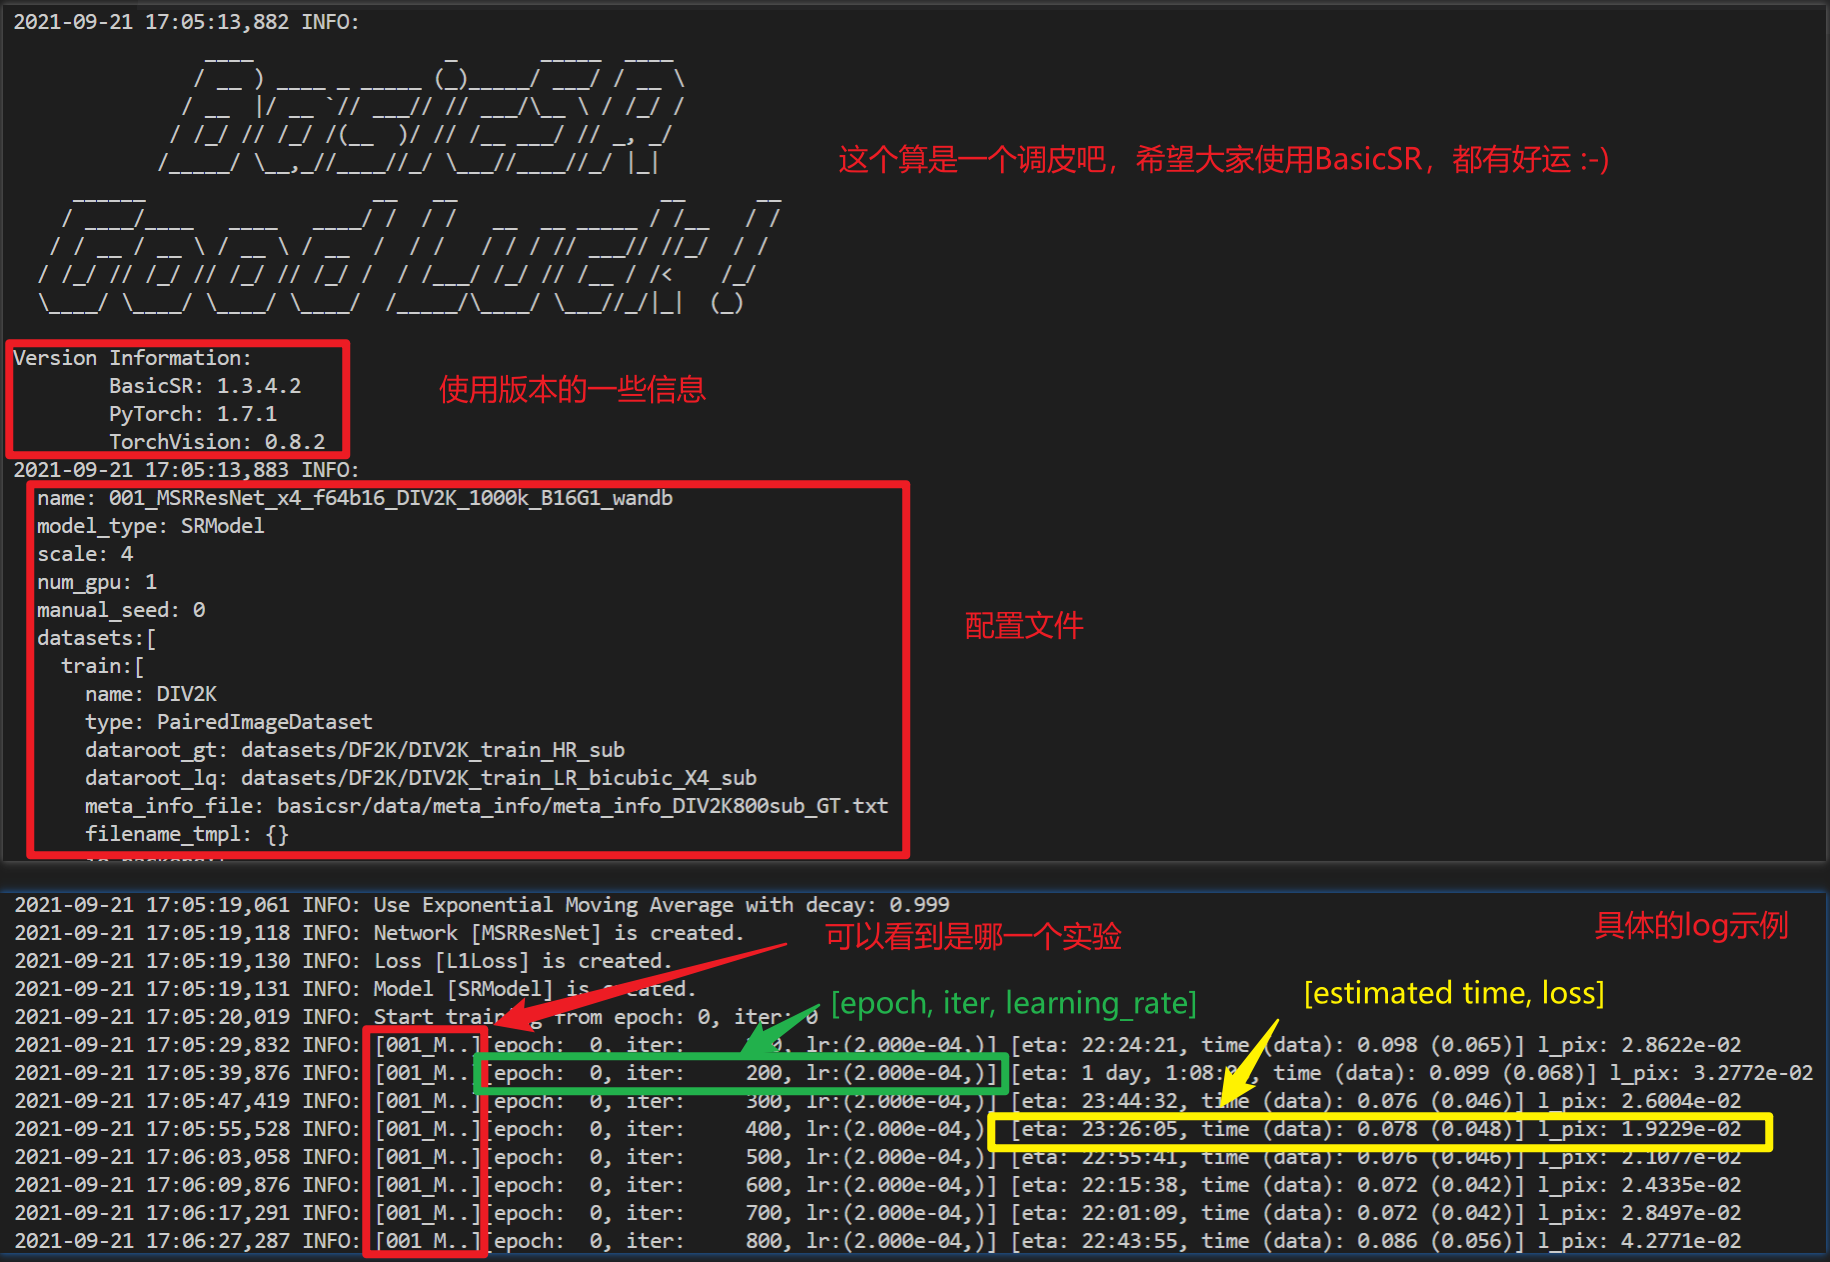
\includegraphics[width=0.9\linewidth]{figures/code_structure_log_example.png}
        \caption{实验过程中产生的 log 信息}
        \label{fig:getting_start_6}
    \end{center}
    \vspace{-0.5cm}
\end{figure}

\begin{minted}[xleftmargin=20pt,linenos,bgcolor=bg,breaklines]{yaml}
# log 文件所在位置: experiments/实验名字/train_[exp_name]_[timestamp].log
2022-06-17 02:27:36,068 INFO:
# 在代码中调用 logger.info()后,会自动记录时间并增加条目 INFO:
# 为节省篇幅,下面 log 中删掉了时间信息

Version Information:
# 软件的版本
    BasicSR: 1.3.3.10
    PyTorch: 1.9.1+cu111
    TorchVision: 0.10.1+cu111
INFO:
  name: 000_SRResNet_DIV2K
  # 实验名,整个 配置option 的内容都会记录在这里,这里省略掉了


INFO: Dataset [XXXDataset] - XXXdata is built.
INFO: Training statistics:
# 训练数据的信息,数量、batchsize 等
    Number of train images: 38684
    Dataset enlarge ratio: 1
    Batch size per gpu: 16
    World size (gpu number): 1
    Require iter number per epoch: 2418
    Total epochs: 207; iters: 500000.
INFO: Dataset [PairedImageDataset] - validation is built.
# dataset 类型
INFO: Number of val images/folders in validation: 14
# 验证集信息
INFO: Network [MSRResNet] is created.
INFO: Network: MSRResNet, with parameters: 1,222,147
# 网络参数量
INFO: MSRResNet(
# 网络结构,此处省略

INFO: Use Exponential Moving Average with decay: 0.999
INFO: Loss [L1Loss] is created.
INFO: Model [RealESRNetModel_XXX] is created.
INFO: Start training from epoch: 0, iter: 0
# 开始训练
INFO: [001_M..][epoch:  0, iter:     100, lr:(2.000e-04,)] [eta: 2 days, 21:55:41, time (data): 0.040 (0.004)] l_pix: 5.0581e-02
# [001_M..]: 实验名字,推荐使用数字打头的实验名,这样可以很方便区分实验
# [epoch: 第几轮, iter: 第几次迭代 (一次迭代是一个batch), lr:学习率 (如果分组,则会显示多组)]
# [eta:预估剩余时间, time (data):一次迭代所需时间 (读取数据的时间)]
# l_pix: 当前的各项 loss

INFO: Validation validation
# 验证集验证结果
     #  psnr: 18.0289

INFO: End of training. Time consumed: 10:22:17
INFO: Save the latest model.
INFO: Validation validation
# 训练结束,最终验证集结果
     #  psnr: 20.7466
\end{minted}

% ----------------------------------
\subsection{tensorboard logger 记录及解读}

除了上述的 log 文件外,BasicSR 还会生成可以用 tensorboard 打开的 tb\_logger 文件。一般保存在 BasicSR/experiments/tb\_logger/实验名。


如何开启: 在 yml 配置文件中设置 `\texttt{use\_tb\_logger: true}':
\begin{minted}[xleftmargin=20pt,linenos,bgcolor=bg,breaklines]{python}
# yml
    logger:
      use_tb_logger: true
\end{minted}

在命令行输入以下命令,就可以在浏览器中查看:
\begin{minted}[xleftmargin=20pt,linenos,bgcolor=bg,breaklines]{bash}
tensorboard --logdir tb_logger --port 5500 --bind_all
\end{minted}

下图\ref{fig:tensorboard_demo}是一个示例:
\begin{figure}[h]
    %\vspace{-0.5cm}
    \begin{center}
        %\fbox{\rule{0pt}{2.5in} \rule{0.9\linewidth}{0pt}}
        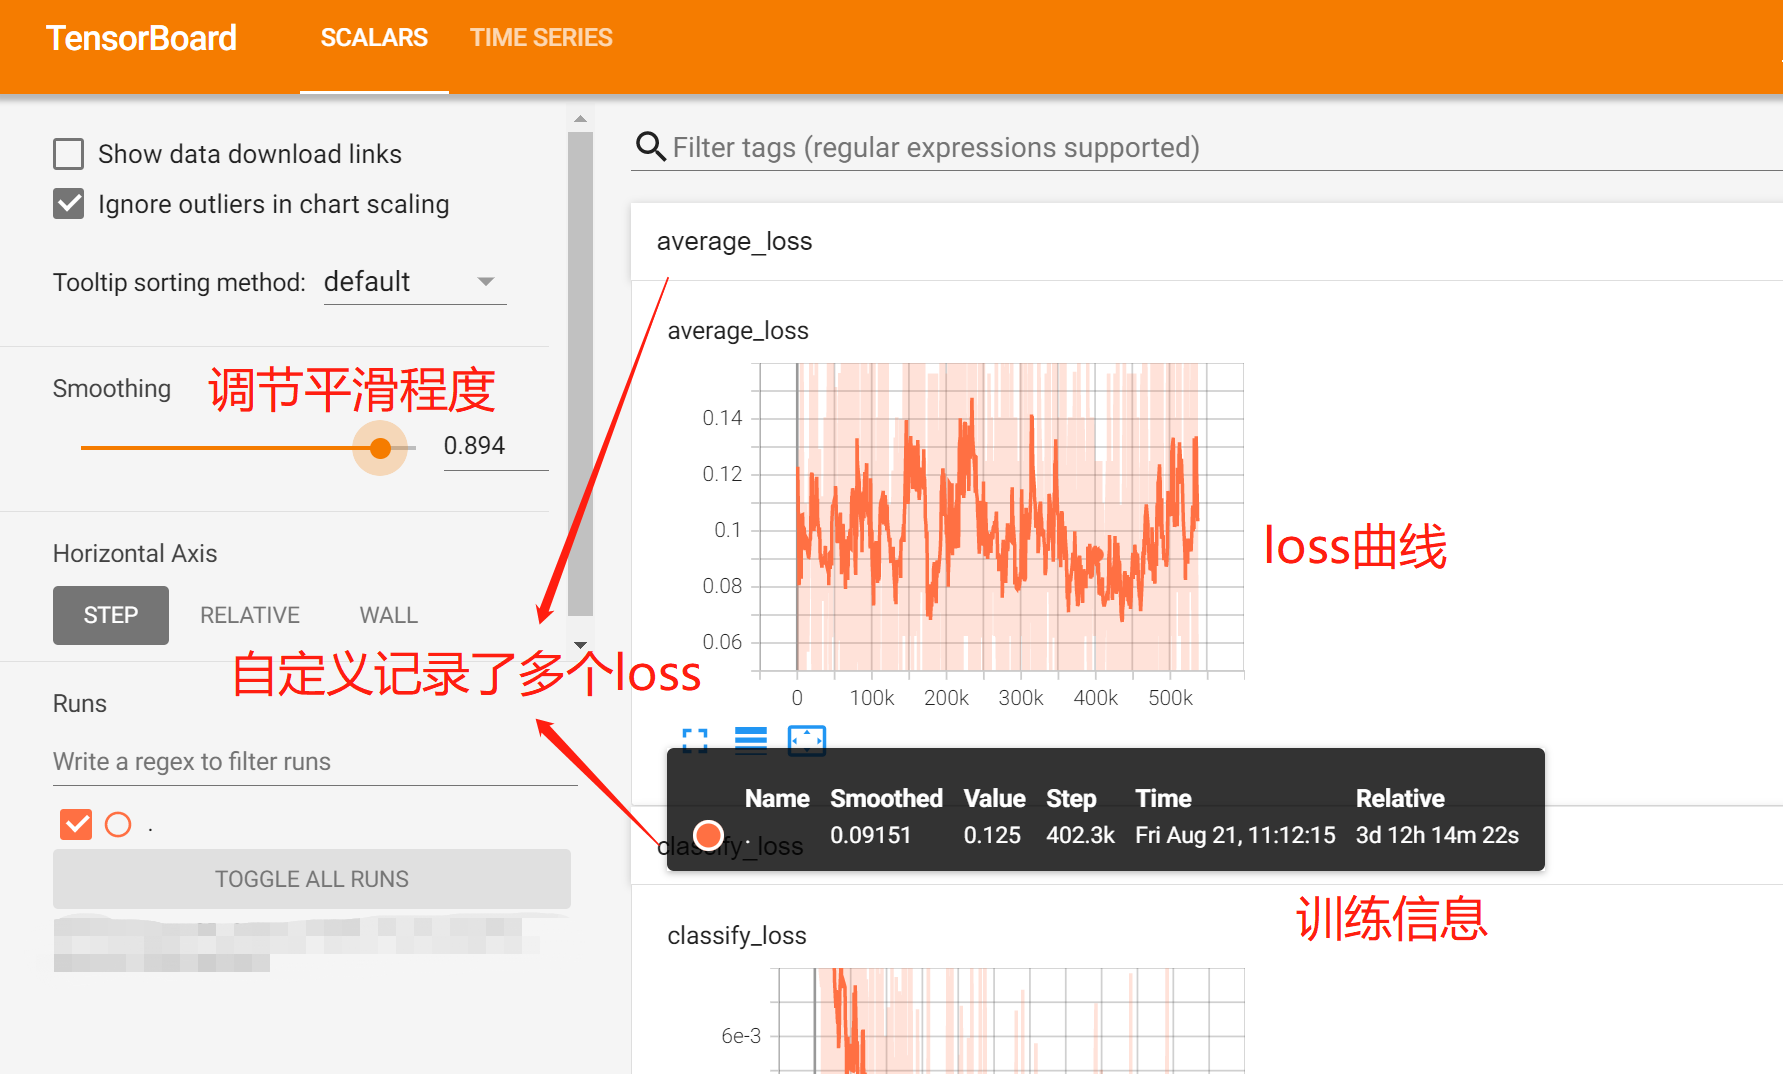
\includegraphics[width=0.8\linewidth]{figures/code_structure_tensorboard.png}
        % \vspace{-1cm}
        \caption{tensorboard示例图}
        \label{fig:tensorboard_demo}
    \end{center}
    %\vspace{-0.7cm}
\end{figure}

目前 BasicSR 里 tb\_logger 主要记录 validation 结果和训练过程中的 loss。validation 结果会随着 metric 而增加,不过多赘述。重点介绍如何添加 loss 记录到 tb\_logger 。

\begin{hl} % ---------------- Highlight block ---------------- %
    虽说封装的很深,但是实际在框架中使用起来,只需要在 xx\_model.py 计算 loss 之后,执行 \texttt{loss\_dict['新的loss'] = 新的loss} ,即可同时记录在 tb\_logger 和 log 文件中。

    注意:也可以使用这种方法记录不是 loss 的其他值。
\end{hl}

\begin{exampleBox}[righthand ratio=0.00, sidebyside, sidebyside align=center, lower separated=false]{log 命名的约定}
在 log 的时候, loss 项使用 l\_ 开头,这样在 Tensorboard 显示的时候,所有 loss 会被组织到一起。比如在 \href{https://github.com/XPixelGroup/BasicSR/blob/master/basicsr/models/srgan_model.py}{basicsr/models/srgan\_model.py} 中,使用了 l\_g\_pix,l\_g\_percep,l\_g\_gan 等。在 \href{https://github.com/XPixelGroup/BasicSR/blob/master/basicsr/utils/logger.py}{basicsr/utils/logger.py} 中,他们会被组织到一起:
\begin{minted}[xleftmargin=20pt,bgcolor=bg,breaklines]{python}
if k.startswith('l_'):
    self.tb_logger.add_scalar(f'losses/{k}', v, current_iter)
else:
    self.tb_logger.add_scalar(k, v, current_iter)
\end{minted}
\end{exampleBox}

下面介绍具体的封装细节,tb\_logger 的初始化和记录代码为:

\begin{minted}[xleftmargin=20pt,linenos,bgcolor=bg,breaklines]{python}
# 这个是记录validation结果的
tb_logger.add_scalar(f'metrics/{metric}', value, current_iter)

\end{minted}

一个上述语句封装的例子:

\begin{minted}[xleftmargin=20pt,linenos,bgcolor=bg,breaklines]{python}
# BasicSR/basicsr/train.py中:

    tb_logger = init_tb_loggers(opt)
    # 初始化tb_logger
    msg_logger = MessageLogger(opt, current_iter, tb_logger)
    # 实例化msg_logger,包含了tb_logger
    ...
    log_vars.update(model.get_current_log())
    # 更新log_vars
    msg_logger(log_vars)
    # 调用messagelogger

# BasicSR/basicsr/utils/logger.py中定义了MessageLogger类:

    class MessageLogger():
        ...
        def __call__(self, log_vars):
            ...
            self.tb_logger.add_scalar(f'losses/{k}', v, current_iter)
            # 这里调用了添加tb_logger

# BasicSR/basicsr/models/base_model.py中定义了get_current_log():

    def get_current_log(self):
        return self.log_dict

# self.log_dict在BasicSR/basicsr/models/sr_model.py中:

    loss_dict['l_pix'] = l_pix
    self.log_dict = self.reduce_loss_dict(loss_dict)
\end{minted}



% ----------------------------------
\subsection{Wandb 记录及解读}

\href{https://www.wandb.com/}{wandb} 类似tensorboard的云端版本, 可以在浏览器方便地查看模型训练的过程和曲线。我们目前只是把tensorboard的内容同步到wandb上, 因此要使用wandb, 必须打开tensorboard logger,参见上一节。\href{https://wandb.ai/xintao/basicsr?workspace=user-}{BasicSR wandb示例}

配置文件如下:
\begin{minted}[xleftmargin=20pt,linenos,bgcolor=bg,breaklines]{python}
yml
logger:
  # 是否使用tensorboard logger
  use_tb_logger: true
  # 是否使用wandb logger,目前wandb只是同步tensorboard的内容,因此要使用wandb, 必须也同时使用tensorboard
  wandb:
    # wandb的project. 默认是 None, 即不使用wandb.
    # 这里使用了 basicsr wandb project: https://app.wandb.ai/xintao/basicsr project: basicsr
    # 如果是resume, 可以输入上次的wandb id, 则log可以接起来
    resume_id: ~
\end{minted}

\end{document}
